% $Header: /Users/joseph/Documents/LaTeX/beamer/solutions/conference-talks/conference-ornate-20min.en.tex,v 90e850259b8b 2007/01/28 20:48:30 tantau $

\documentclass[aspectratio=169]{beamer}

% This file is a solution template for:

% - Talk at a conference/colloquium.
% - Talk length is about 20min.
% - Style is ornate.



% Copyright 2004 by Till Tantau <tantau@users.sourceforge.net>.
%
% In principle, this file can be redistributed and/or modified under
% the terms of the GNU Public License, version 2.
%
% However, this file is supposed to be a template to be modified
% for your own needs. For this reason, if you use this file as a
% template and not specifically distribute it as part of a another
% package/program, I grant the extra permission to freely copy and
% modify this file as you see fit and even to delete this copyright
% notice. 


\mode<presentation>
{
  \usetheme{Madrid}
  % or ...

  \setbeamercovered{transparent}
  % or whatever (possibly just delete it)
}

\frenchspacing
% or whatever

\usepackage[utf8]{inputenc}
% or whatever


\usepackage{times}
\usepackage[T1]{fontenc}
% Or whatever. Note that the encoding and the font should match. If T1
% does not look nice, try deleting the line with the fontenc.

\title{Workshop: ``Decoding Interplanetary Spacecraft''}

\author{Dr. Daniel Est\'evez}


\institute
{}
% - Use the \inst command only if there are several affiliations.
% - Keep it simple, no one is interested in your street address.

\date % (optional, should be abbreviation of conference name)
[GRCon20, September 2020]{14 September 2020\\\vspace{1em}
\includegraphics[width=3cm]{grcon20}}
% - Either use conference name or its abbreviation.
% - Not really informative to the audience, more for people (including
%   yourself) who are reading the slides online

\subject{}
% This is only inserted into the PDF information catalog. Can be left
% out.

% If you have a file called "university-logo-filename.xxx", where xxx
% is a graphic format that can be processed by latex or pdflatex,
% resp., then you can add a logo as follows:

% \pgfdeclareimage[height=0.5cm]{university-logo}{university-logo-filename}
% \logo{\pgfuseimage{university-logo}}



% Delete this, if you do not want the table of contents to pop up at
% the beginning of each subsection:
\AtBeginSection[]
{
  \begin{frame}<beamer>{Outline}
    \tableofcontents[currentsection,currentsubsection]
  \end{frame}
}


% If you wish to uncover everything in a step-wise fashion, uncomment
% the following command: 

%\beamerdefaultoverlayspecification{<+->}

\newcommand{\handson}[1]{\begin{frame}
 \begin{block}{}
   \begin{center}
     \vspace{0.5em}
     {\bf Hands-on:} #1
     \vspace{0.5em}
   \end{center}
 \end{block}
 \end{frame}
}


\begin{document}

\begin{frame}
  \titlepage
\end{frame}

\begin{frame}{Introduction}
  In this workshop:

  \begin{itemize}
  \item We start off with IQ recordings of some deep-space probes
  \item Use GNU Radio to analyze the signal and find its specs (simple
    reverse-engineering)
  \item Build a decoder to obtain telemetry frames as we go
  \end{itemize}

  Why?
  \begin{itemize}
  \item It is cool!
  \item It isn't difficult: probably easier than your average ASK keyfob
  \item To learn deep-space communications
  \end{itemize}

  The focus is on hands-on with GNU Radio, but there are some slides with the
  theoretical background. You can always come back to these later.
\end{frame}

\begin{frame}{ESA Solar Orbiter}
  \begin{center}
    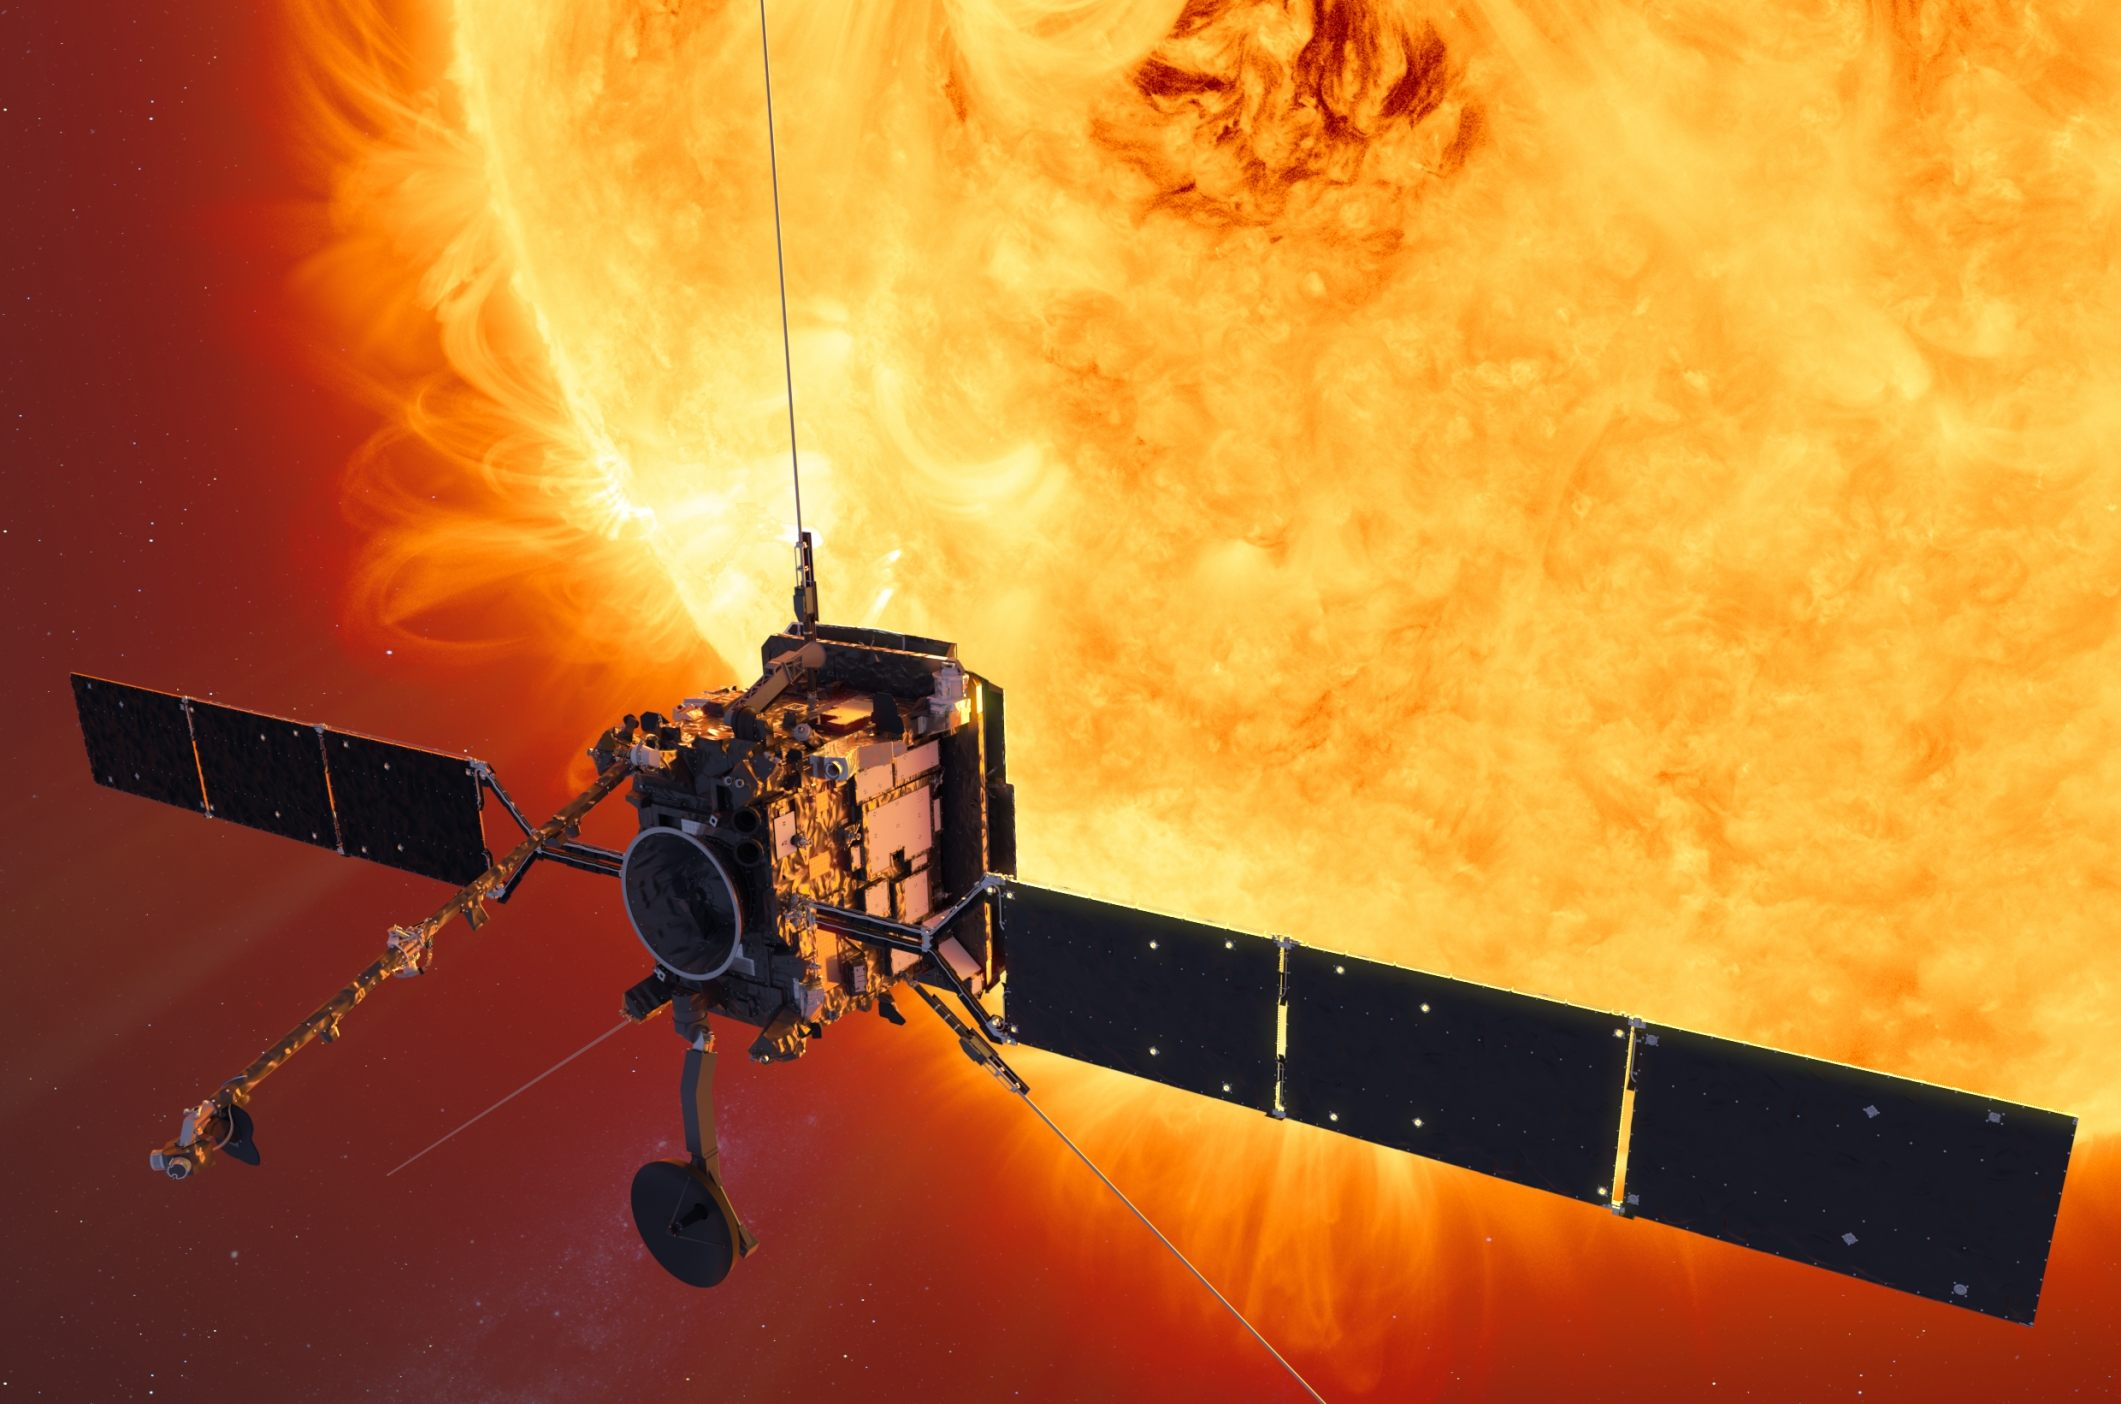
\includegraphics[width=8cm]{solar_orbiterTHUMB}
  \end{center}

  ESA mission to study the heliosphere and solar wind (some participation of NASA)
  
  Launched on 10 February 2020

  \begin{flushright}
    {\tiny * Image from ESA Science \& Exploration}
  \end{flushright}
\end{frame}

\begin{frame}{BepiColombo}
   \begin{center}
     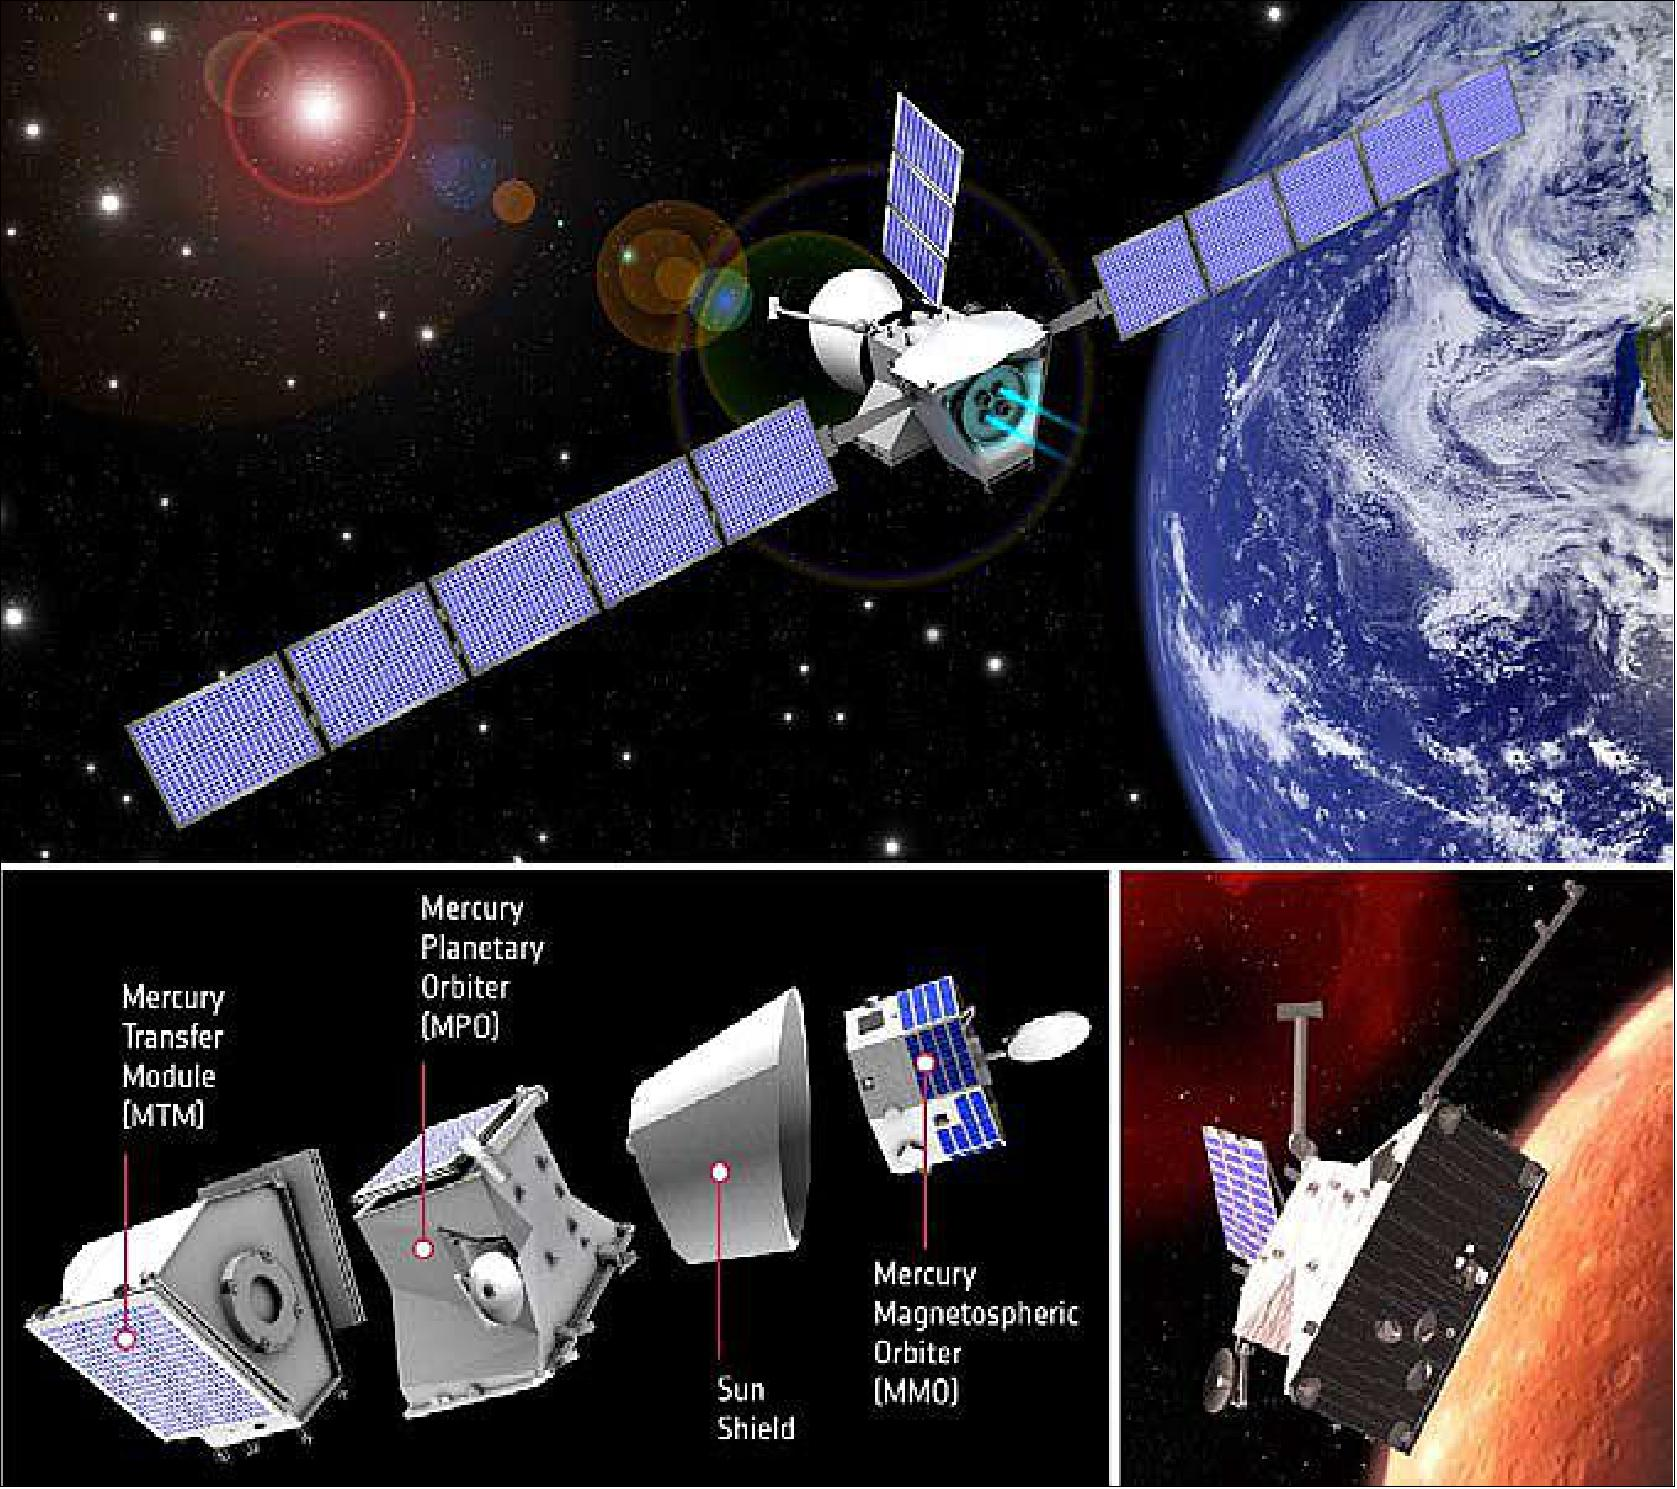
\includegraphics[width=6.1cm]{BepiColombo_Auto6F}
   \end{center}

   ESA / JAXA mission to Mercury

   Launched on 20 October 2018, Earth flyby on 10 April 2020

   \begin{flushright}
    {\tiny * Image from eoPortal Directory}
  \end{flushright}
\end{frame}

\begin{frame}{Receiving deep-space probes signals}
  These spacecraft transmit telemetry in the X band, around 8.4GHz

  \medskip
  
  The signal can be detected with ``small'' dishes from long distances, but to
  have enough SNR to demodulate the data, the spacecraft needs to be near Earth

  \medskip
  
  The recordings used here have been made by Paul Marsh M0EYT:

  \begin{itemize}
  \item Solar Orbiter: 3 days after launch, 1.7 million km away
  \item BepiColombo: 6 days before Earth flyby, 2 million km away
  \end{itemize}

  More is possible: Paul is currently demodulating Tianwen-1 at 16 million km on
  its way to Mars

  \medskip

  Put these numbers in perspective: the Earth-Moon distance is 0.4 million km;
  light takes 10 seconds to travel 3 million km
  
\end{frame}

\begin{frame}
  This is Paul's 2.4m antenna.

  \begin{center}
    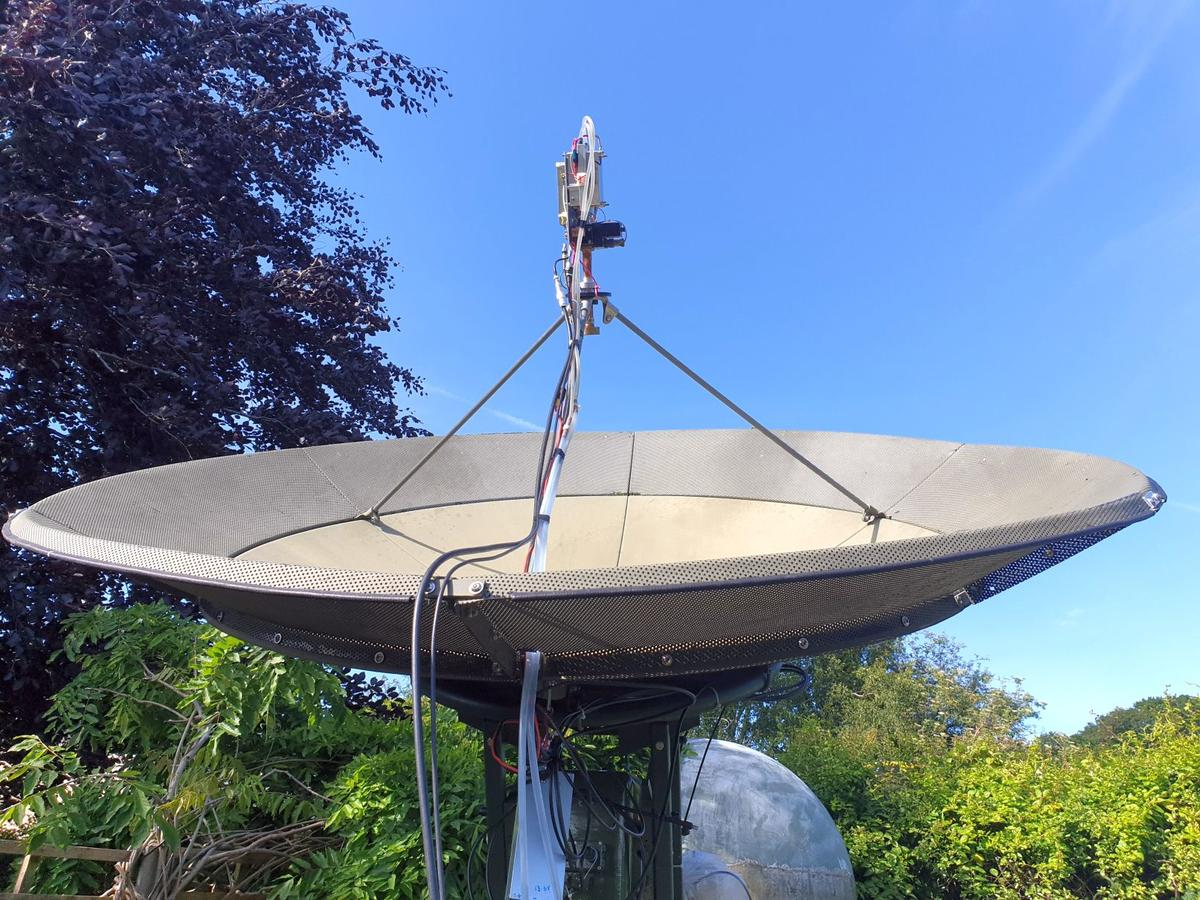
\includegraphics[width = 9.5cm]{10gemedish1}
  \end{center}
\end{frame}

\begin{frame}{Signal spectrum}
  The first step in analyzing a signal is looking at the spectrum and/or waterfall

  This requires computing FFTs to pass from time domain to frequency domain

  \medskip

  The \emph{QT GUI Frequency Sink} and \emph{QT GUI Waterfall Sink} GNU Radio
  blocks can be used for this

  \medskip

  inspectrum, by Mike Walters is also a good tool for viewing the waterfall of a
  recording

  \url{https://github.com/miek/inspectrum}
\end{frame}

\handson{Visualizing the spectrum}

\begin{frame}{Phase modulation in deep-space communications}
  Many deep-space comms systems use residual-carrier phase modulation:

  \[
  x(t) = A\cos(2 \pi f_0 t + \varphi(t)) =
  \operatorname{Re}(x_{BB}(t) \exp(2 \pi i f_0 t)),\quad x_{BB}(t) = A\exp(i \varphi(t))
  \]

  \[
  \varphi(t) = D s(t) d(t), \quad s(t) = h(\sin(2 \pi f_{sc} t + \varphi_{sc})),
  \quad d(t) = \sum_{n \in \mathbb{Z}} d_n p(t/T_s - n),
  \]

  where $D$ is the deviation,
  $h(t) = t$ for a sine-wave subcarrier, $h(t) = \operatorname{sign}(t)$
  for a square-wave subcarrier, $d_n = \pm 1$, and $p$ is the data pulse shaping
  filter, typically $p(t) = 1$ for $0 \leq t \leq 1$, and $p(t) = 0$ otherwise.

  \medskip

  Manchester encoding is a special case, where $h(t) =
  \operatorname{sign}(t)$, $f_{sc} = 1/T_s$ and $\varphi_{sc} = 0$.
  
  \medskip
  
  The residual carrier can be used to recover the carrier phase

  \medskip

  Suppressed-carrier modulations, such as GMSK/OQPSK are also possible,
  especially for high-speed data
\end{frame}

\begin{frame}{Spectrum depending on the subcarrier}
  The subcarrier can be used to push the data power away from the suppressed
  carrier, to help suppressed carrier recovery with a PLL

  There are the following possibilities:
  \begin{itemize}
  \item Subcarrier, $f_{sc} > 1/T_s$
  \item Manchester encoding, $f_{sc} = 1/T_s$
  \item Baseband modulation, $s(t) = 1$ ($f_{sc} = 0$)
  \end{itemize}
  
\begin{center}
  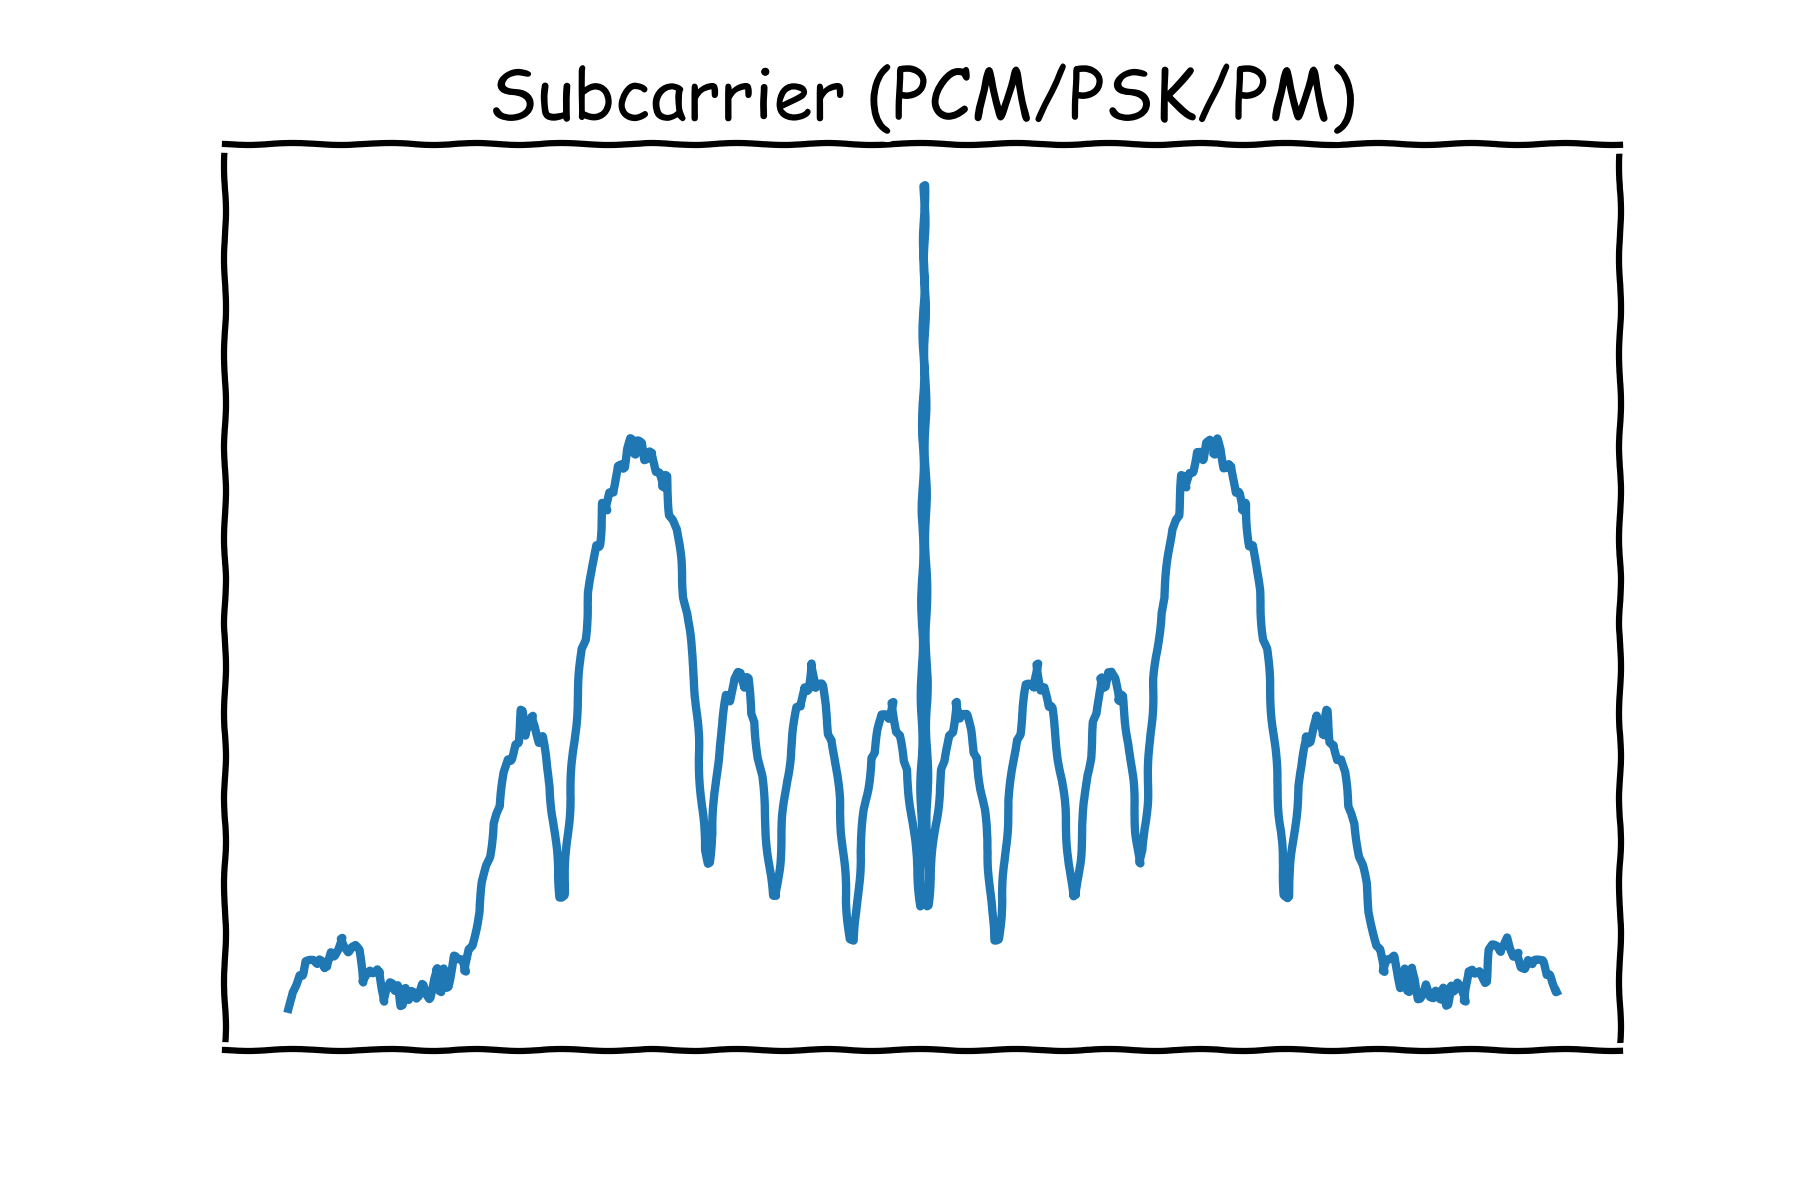
\includegraphics[width=5cm]{subcarrier}
  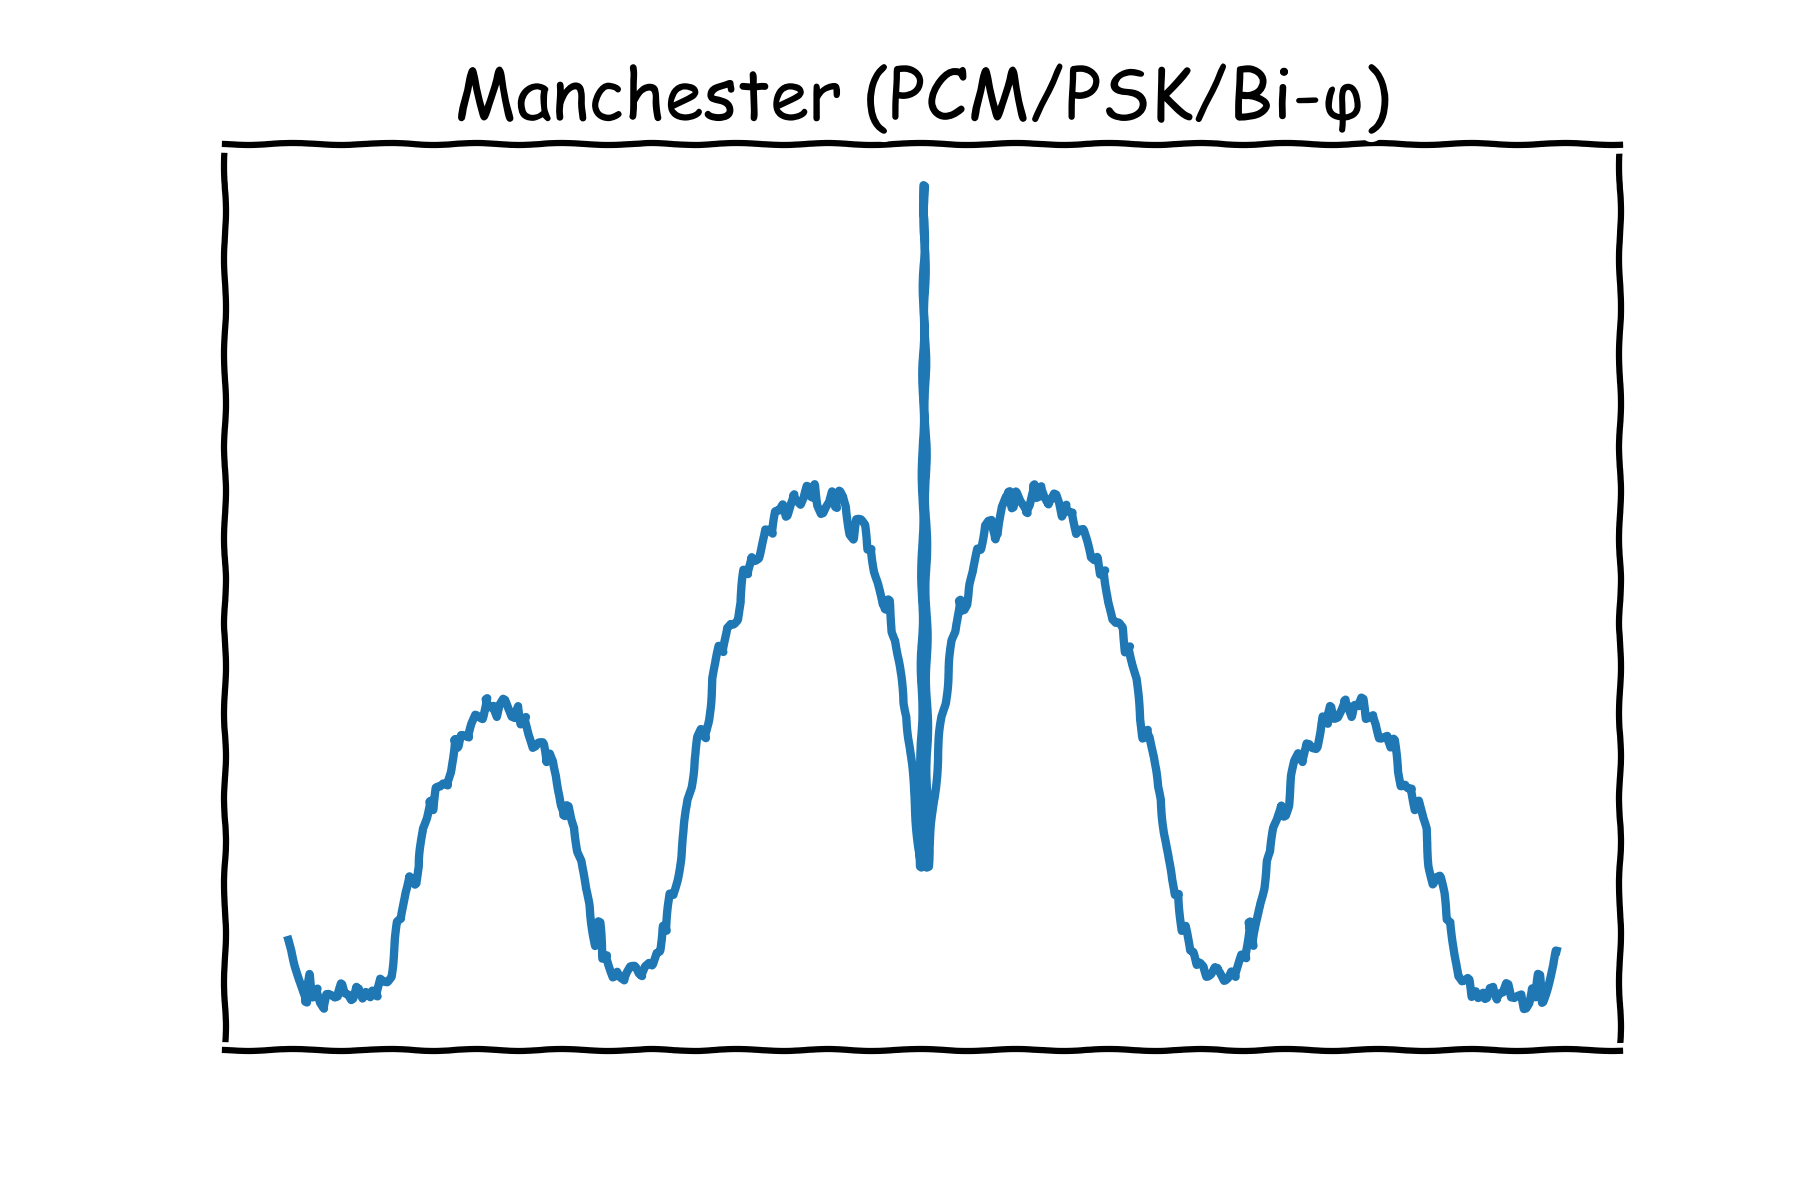
\includegraphics[width=5cm]{manchester}
  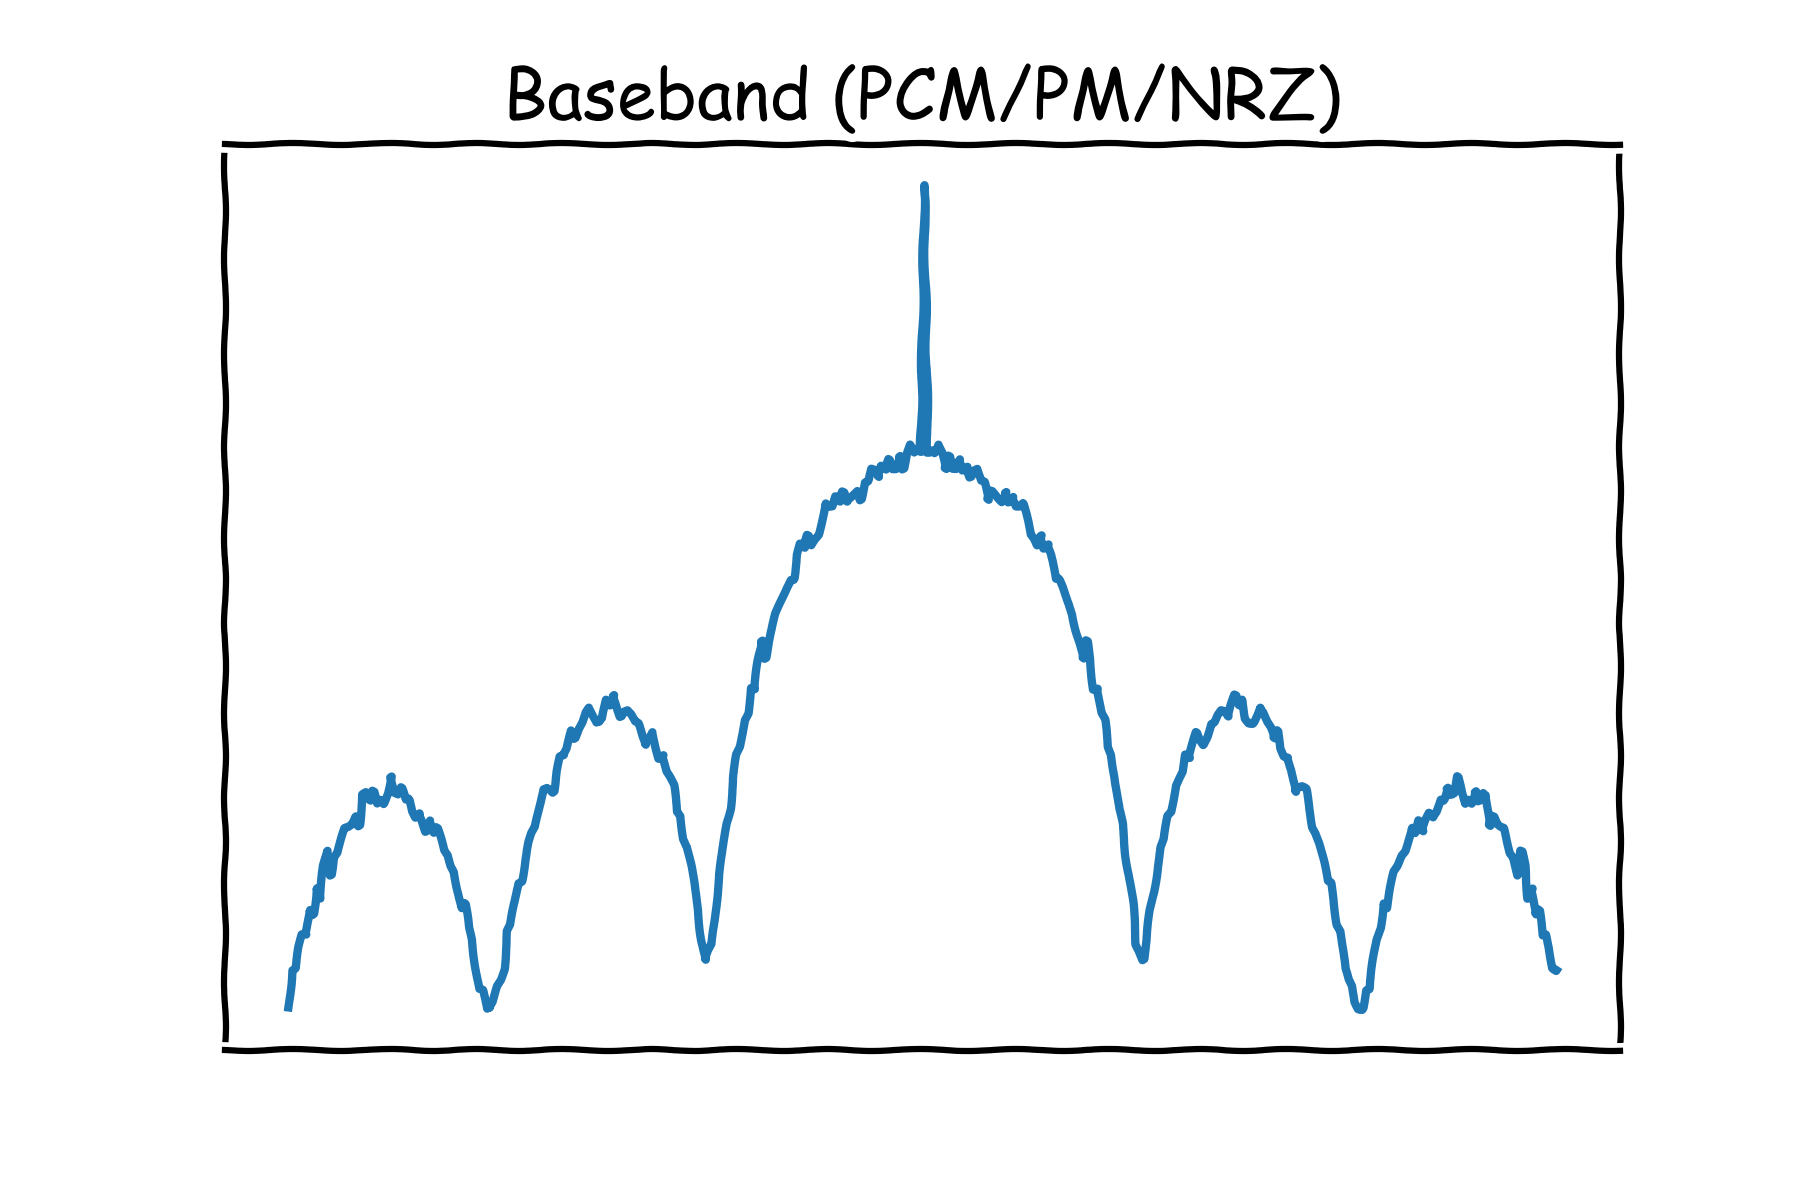
\includegraphics[width=5cm]{baseband}
\end{center}
\end{frame}

\begin{frame}{Carrier phase recovery}
  We use a PLL to recover the phase of the residual carrier. Given
  \[
  y(t) = a(t) e^{i\psi(t)} [1 + z(t)] + n_1(t),
  \]
  with $|a'(t)|$, $|\psi'(t)|$, $|\psi''(t)|$ small, a PLL produces an estimate
  $\widehat{\psi} \approx \psi$. Here $\psi$ accounts for the transmitter and
  receiver local oscillator difference and changes in propagation path.

  \medskip

  The \emph{PLL Carrier Tracking} GNU Radio block outputs
  \[
  e^{-i\widehat{\psi}(t)} y(t) \approx a(t)[1 + z(t)] + n_2(t).
  \]
  There are other PLL blocks in GNU Radio which output different things

  \medskip
  
  The PLL blocks (and many others) assume a signal amplitude of one
  ($a(t) \approx 1$), so they are typically used after an AGC. The \emph{RMS AGC}
  block from gr-satellites estimates the signal RMS power and divides the signal
  by it.
\end{frame}

\handson{Carrier phase locking with a PLL}

\begin{frame}{Phase modulation and IQ}
  Phase modulation can be approximated by a linear modulation where the data is
  in quadrature with the suppressed carrier, since $\exp(i\varphi(t)) \approx 1
  + i\varphi(t)$

  \begin{center}
    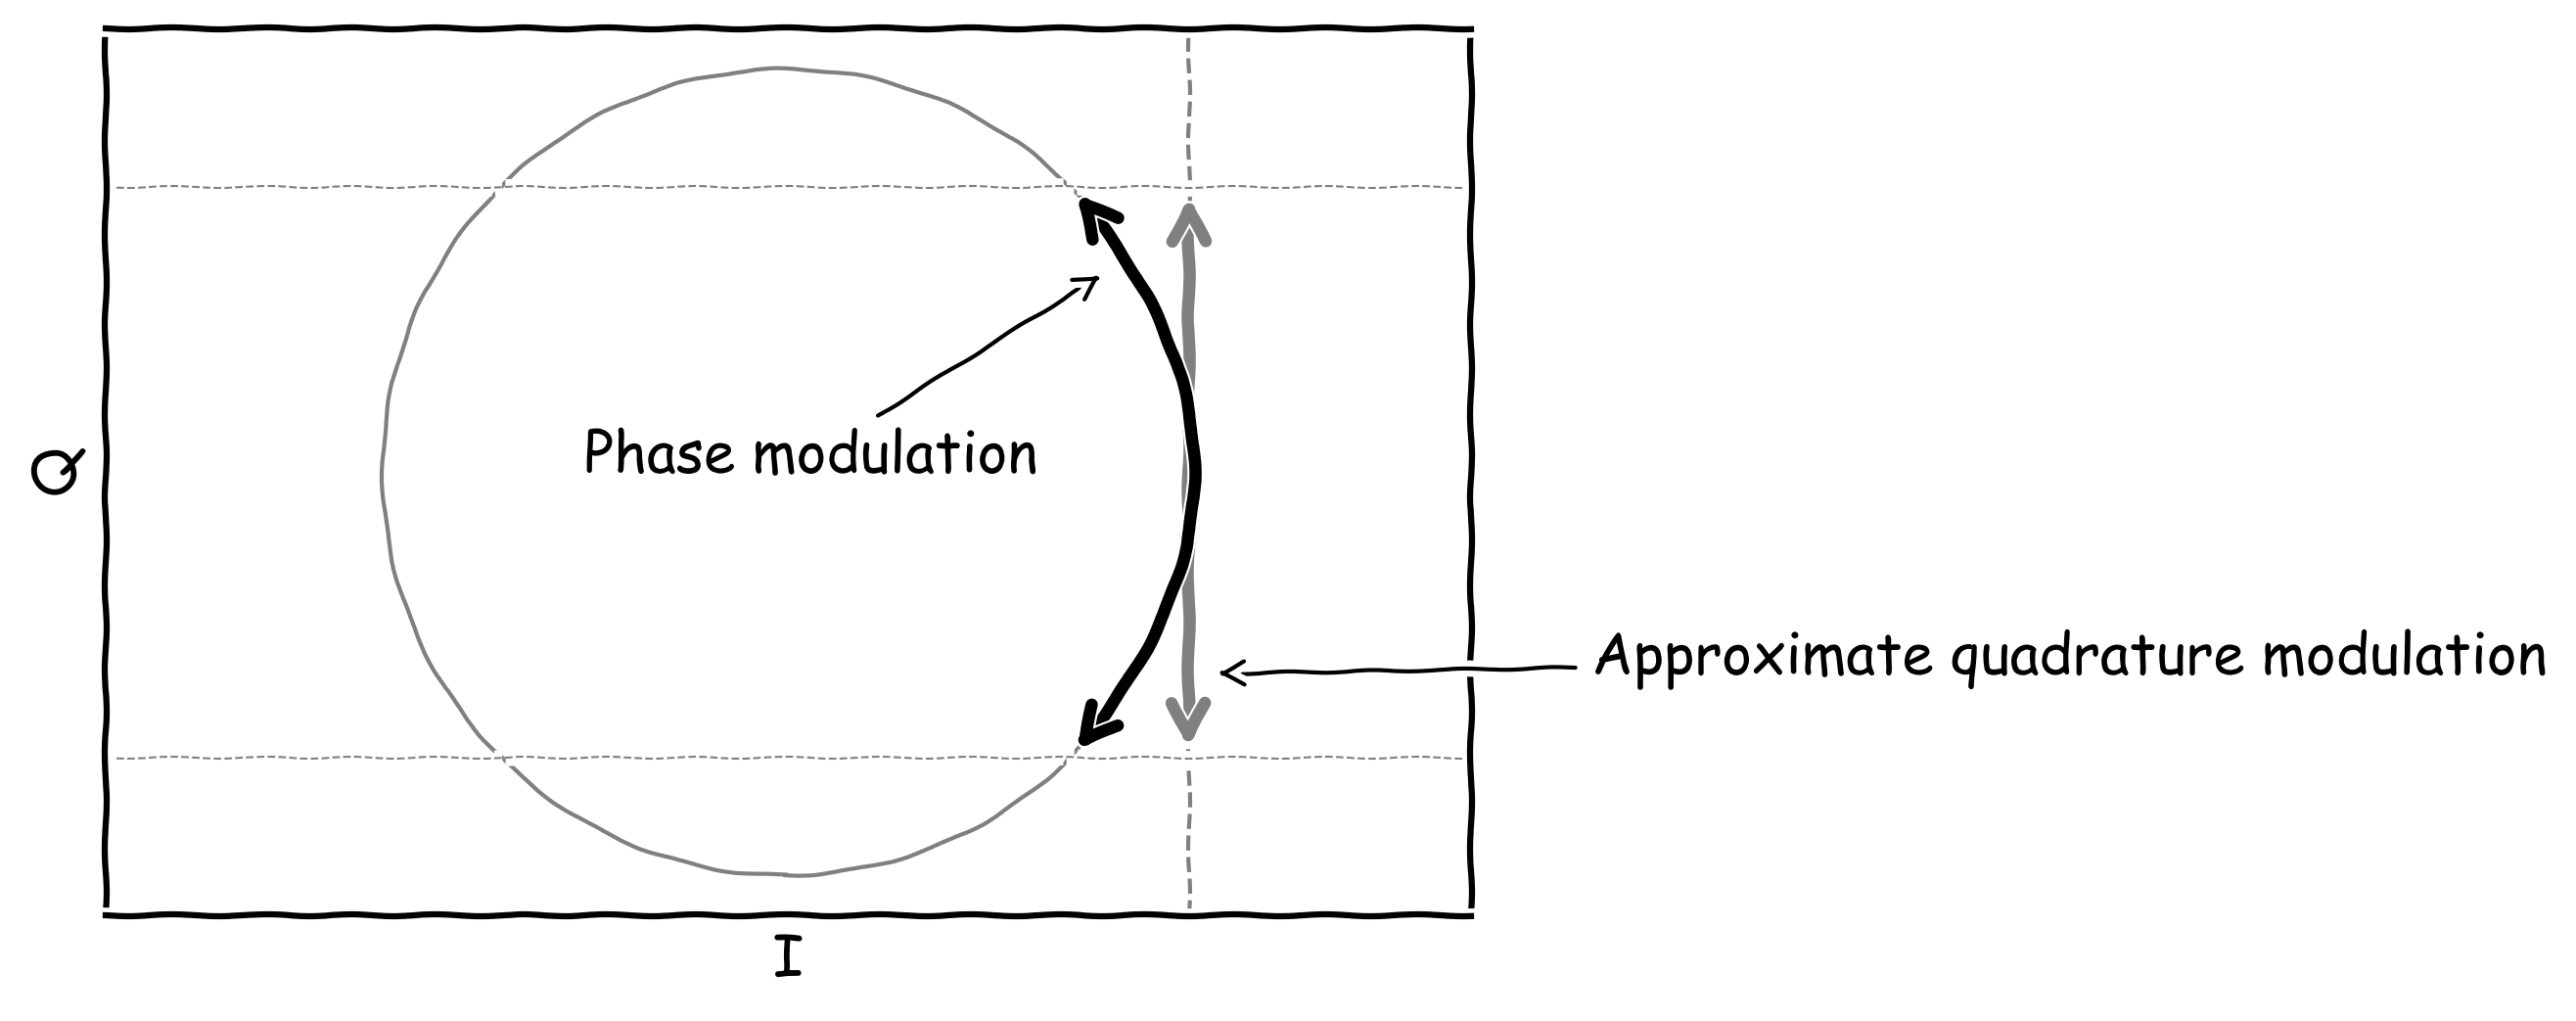
\includegraphics[width=15cm]{iq}
  \end{center}
\end{frame}

\begin{frame}{Downconversion of the data sideband to baseband}
  We take the complex argument (or the imaginary part) at the output of the PLL
  and obtain the real Manchester signal $\varphi(t)$. This has two
  sidebands. Each of the sidebands looks like BPSK, so we can filter one
  sideband, move to baseband, and process as BPSK.

  We use a Hilbert filter to select only one sideband
  \begin{center}
    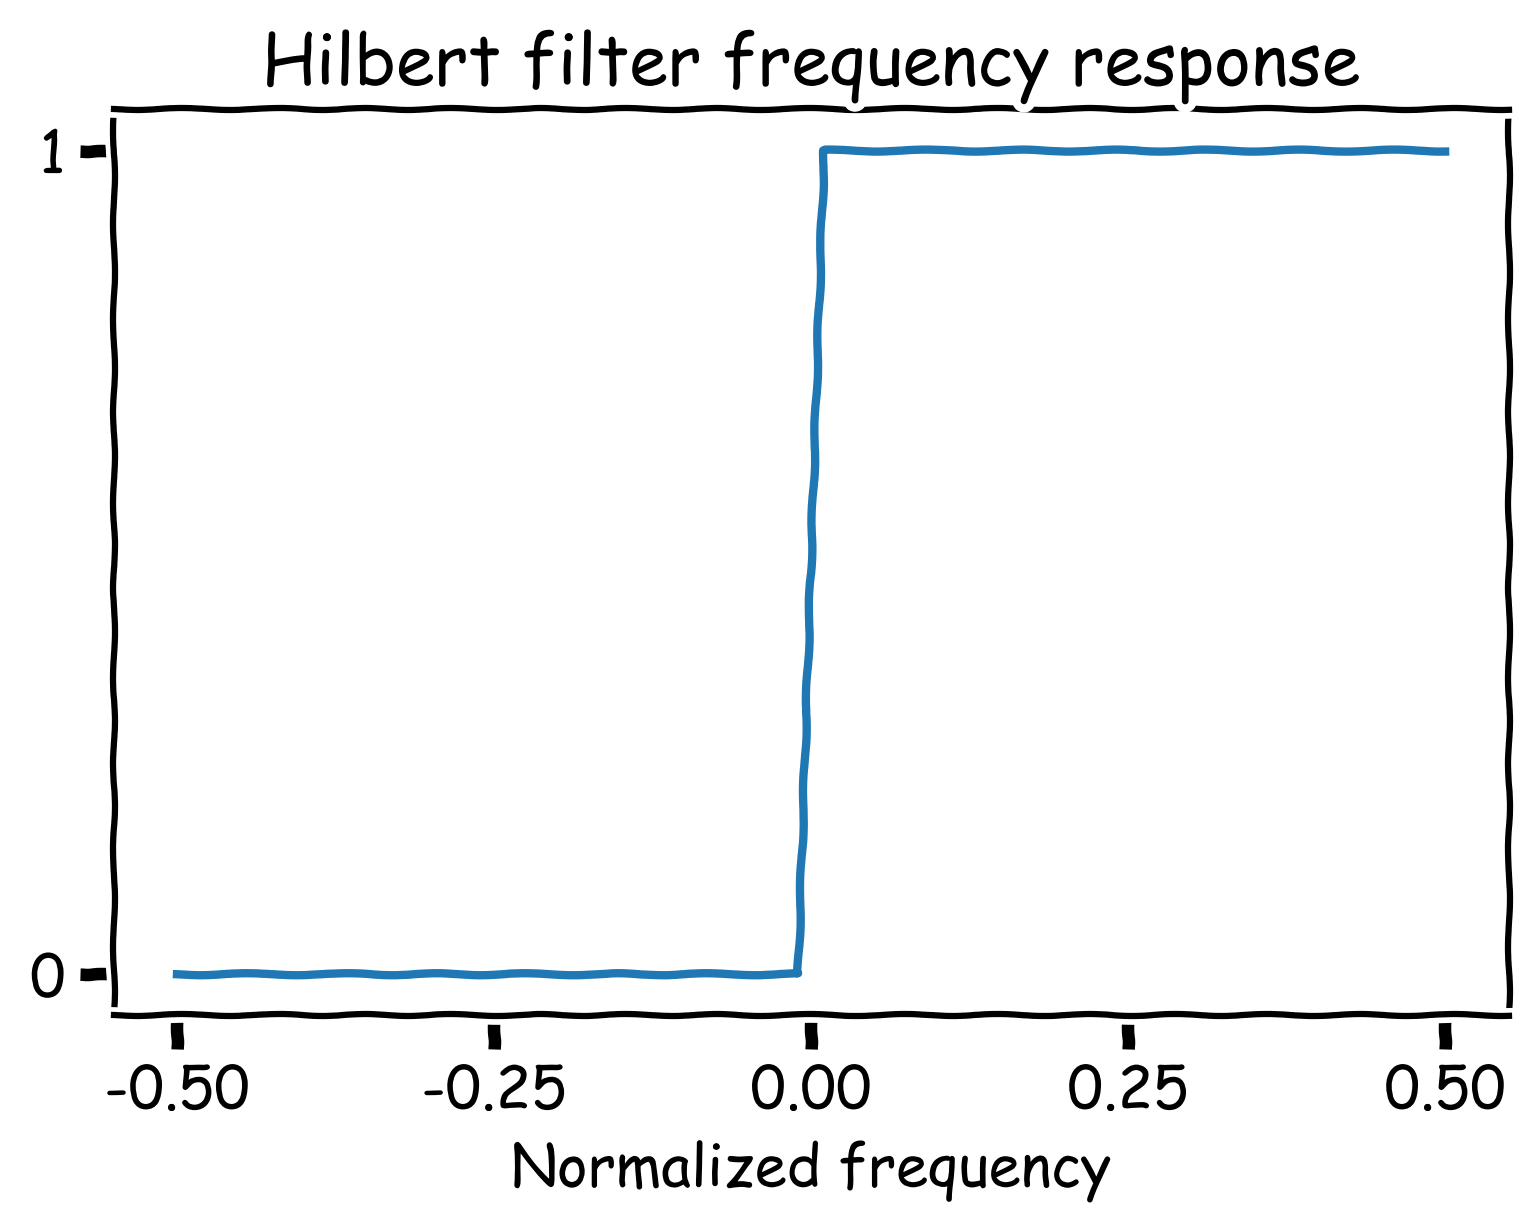
\includegraphics[width=5cm]{hilbert}
  \end{center}

  Then multiply by a complex exponential to move in frequency. Remember:
  multiplication by $\exp(2\pi i f t)$ shifts the frequency by $f$.
\end{frame}

\handson{Downconverting the data sideband to baseband}

\begin{frame}{Finding the carrier frequency of BPSK}
  A BPSK signal is
  \[
  y(t) = d(t)e^{2\pi i f t} + n(t),
  \]
  with $d(t) = \pm 1$. We square it
  \[
  y(t)^2 = e^{4\pi i f t} + 2 n(t) d(t) e^{2\pi i f t}  + n(t)^2
  \]
  and obtain a carrier at frequency $2 f$.

  \medskip

  The same trick can be used for $m$-PSK, by computing the $m$-th power.
\end{frame}

\handson{Refining our downconversion to baseband}

\begin{frame}{Finding the symbol rate}
  We have a BPSK signal in discrete time
  \[
  y[n] = d[n] e^{i \omega n},
  \]
  with $d[n] = \pm 1$. We compute
  \[
  z[n] = y[n] \overline{y[n-1]} = d[n]d[n-1] e^{i \omega}.
  \]
  Then $z[n] = e^{i\omega}$ except when $n-1$ and $n$ lie in different and
  opposite symbols, in which case $z[n] = -e^{i\omega}$.

  \medskip

  So $z[n]$ is a sequence of pulses that occur on some of the symbol changes of
  $y$. The spectrum of $z$ has a strong component at the symbol rate of $y$.

  \medskip
  
  This trick is a simple example of cyclostationary analysis, which is a very
  powerful tool.
\end{frame}

\handson{Finding the symbol rate}

\begin{frame}{Clock recovery}
  We need to filter the noisy BPSK signal with a matched filter to accumulate
  the energy of each symbol and reduce noise. For a square pulse, the matched
  filter is just a moving average. We need to find the optimal sampling
  locations for the symbols. The \emph{Symbol Sync} GNU Radio block will do that
  given an estimate of the symbol rate.

  \begin{center}
    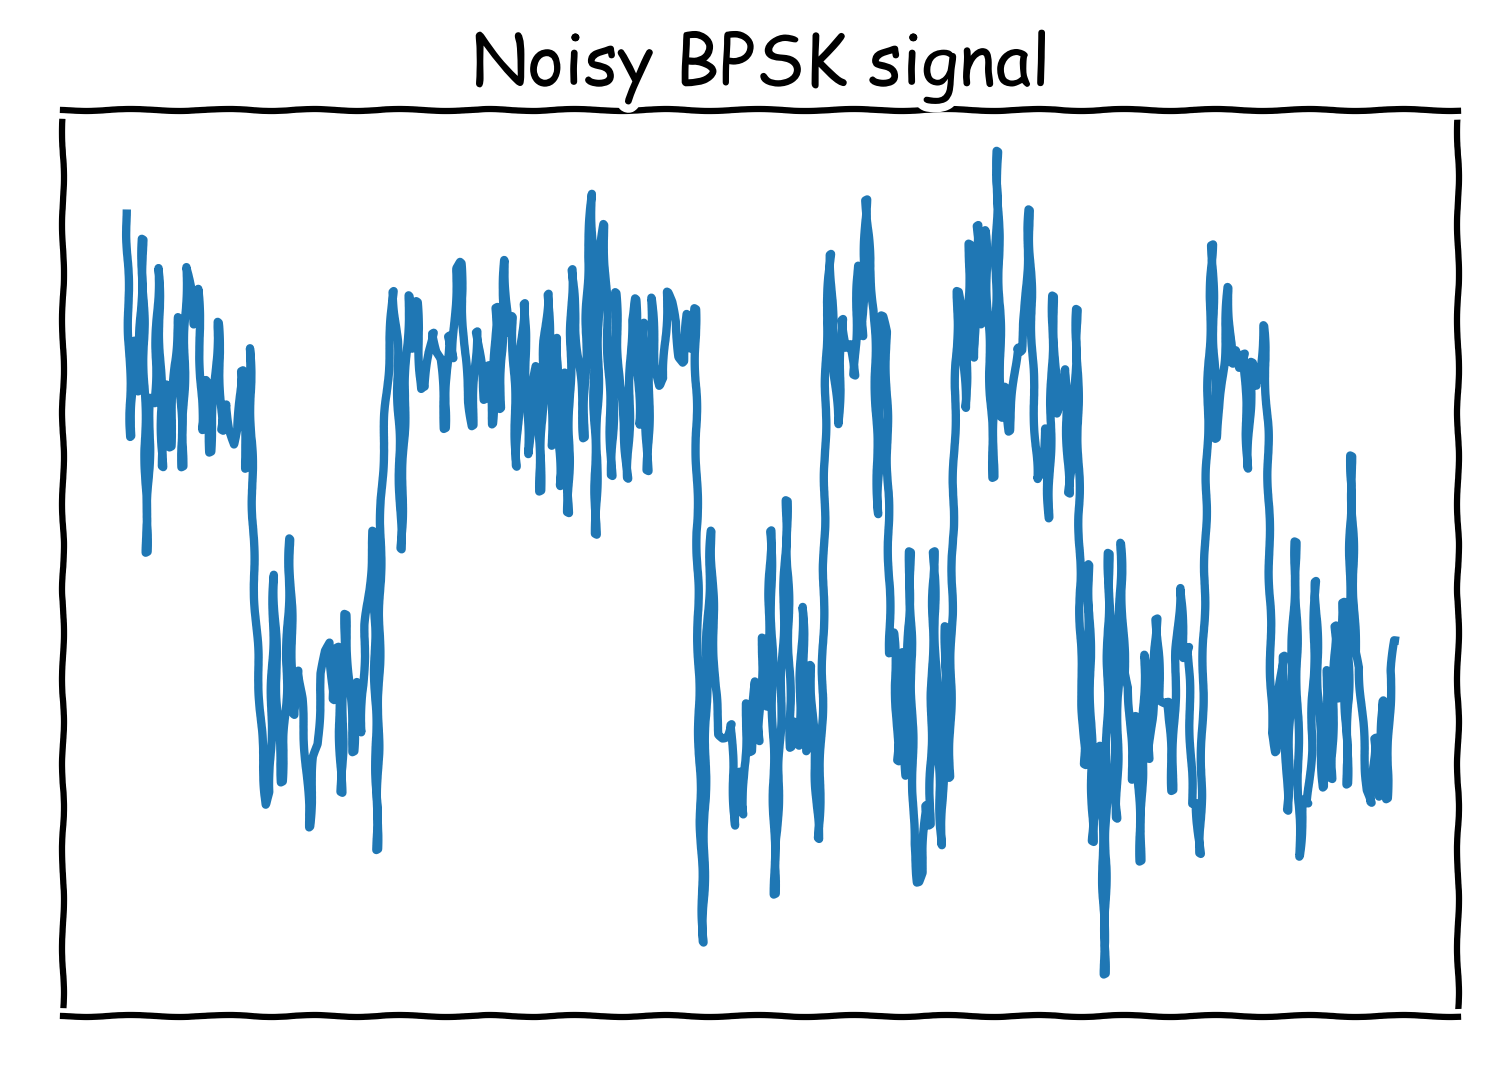
\includegraphics[height=4cm]{pre_matched}
    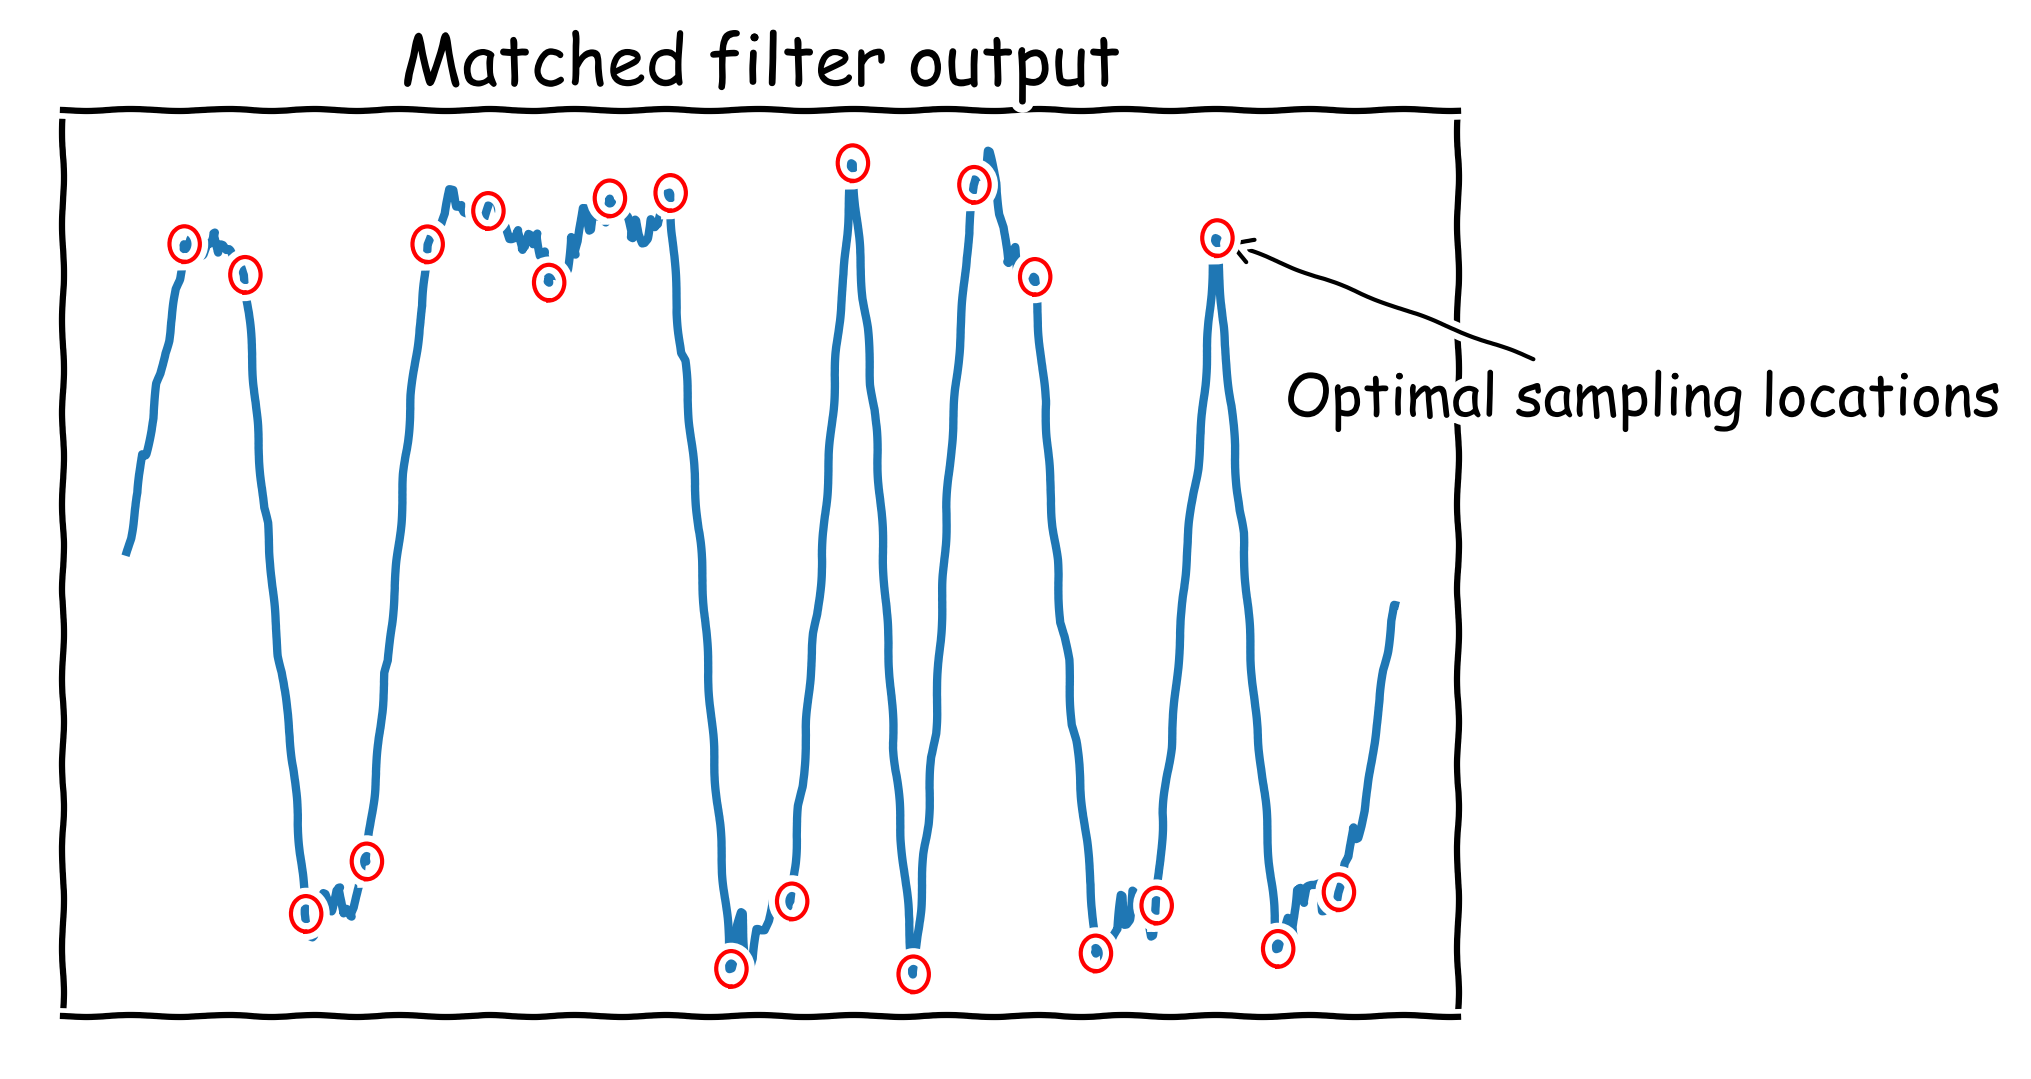
\includegraphics[height=4cm]{post_matched}
  \end{center}
\end{frame}

\begin{frame}{Suppressed carrier recovery}
  After sampling with the \emph{Symbol Sync} block, our symbols look like
  \[S[n] = d_n e^{i\psi_n},\]where $d_n = \pm 1$ and $\psi_n$ changes slowly. We
  still have a suppressed carrier $e^{i\psi_n}$.

  \medskip
  A
  Costas loop will produce an estimate $\widehat{\psi}_n \approx \psi_n$ and
  output
  \[
  e^{-i\widehat{\psi}_n}S[n] \approx d_n.
  \]
  
  \medskip

  There is a 180º phase ambiguity in the Costas loop, so it may happen that
  $\widehat{\psi}_n \approx \psi_n + \pi$ and we get $-d_n$ instead of $d_n$.

  \medskip

  Note that here we are actually using the Costas loop to recover the Manchester
  subcarrier, since the carrier was actually recovered by the PLL.
\end{frame}

\handson{Clock and carrier phase recovery}

\begin{frame}{Coding in deep-space communications: CCSDS}
  Now that we have symbols, we want to decode frames from them

  \medskip
  
  Space communications protocols are standardized by CCSDS in the Blue Books

  The \emph{TM Synchronization and Channel Coding} blue book describes:
  \begin{itemize}
  \item FEC (encode the message to correct bit errors on the receive end)
  \item Scrambling (make the message look random, for performance)
  \item Syncwords (mark the beginning of frames)
  \end{itemize}

  These are the possible types of FEC:
  \begin{itemize}
  \item Convolutional code (Viterbi decoder)
  \item Reed-Solomon
  \item Concatenated (convolutional + Reed-Solomon)
  \item Turbo code
  \item LDPC
  \end{itemize}
\end{frame}

\begin{frame}{CCSDS syncwords}
  The syncword depends on the FEC used. This can help us guess the FEC type.

  \begin{center}
    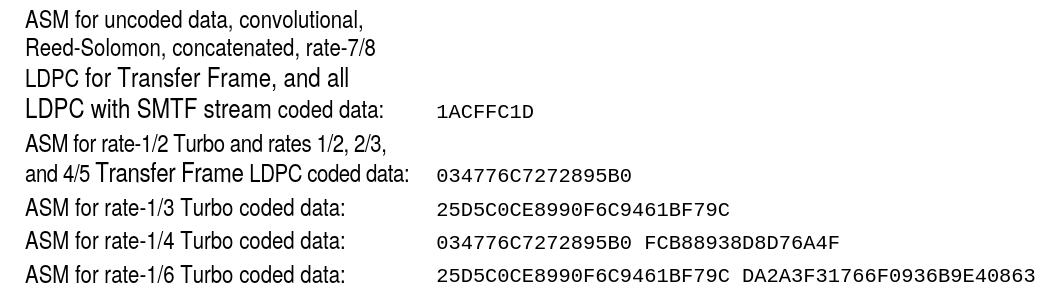
\includegraphics[width=15cm]{syncwords}
  \end{center}

  With convolutional codes, the syncword is sent encoded; with the rest, it is
  sent uncoded

  \medskip

  We can try to correlate the symbol stream against these syncwords. Correlation
  can be implemented by a FIR filter with the \emph{Decimating FIR filter} block.
\end{frame}

\handson{Finding the syncword}

\begin{frame}{Turbo codeword sizes}
  We can find the Turbo code parameters from the codeword size, which can be
  measured from the distance between syncwords

  \begin{center}
    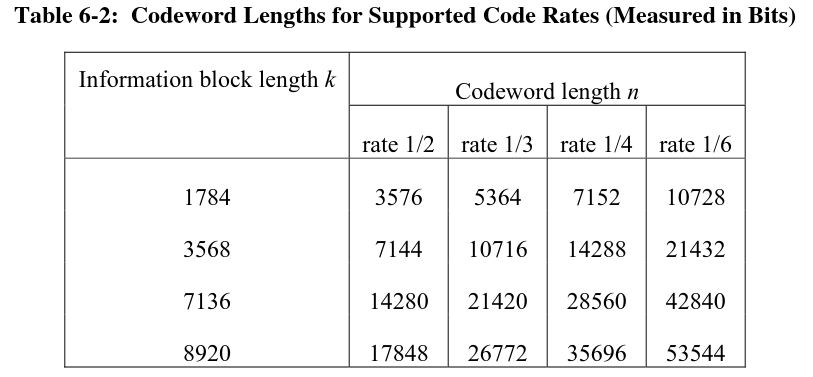
\includegraphics[width=10cm]{codewords}
  \end{center}

  We use \emph{Correlate Access Code - Tag} to detect syncwords (add tags)
  and \emph{Tag debug} to print their locations
\end{frame}

\handson{Finding the codeword size}

\begin{frame}{Turbo decoding with GNU Radio}
  We can use the Turbo decoder blocks from gr-dslwp (Longjiang-2 Chinese lunar
  microsatellite mission) by Wei Mingchuan from Harbin Institute of Technology (China)

  This uses an open source Turbo code implementation by
  Gianluca Marcon, made in 2017 as a course project in Univ.~of Padova (Italy)

  \begin{itemize}
  \item gr-dslwp for GNU Radio 3.8 \url{https://github.com/daniestevez/gr-dslwp/tree/maint38}
  \item Gianluca's deepspace-turbo \url{https://github.com/geeanlooca/deepspace-turbo}
  \end{itemize}
  
  We use:
  \begin{itemize}
  \item \emph{Frame Splitter F} to put each codeword in a PDU
  \item \emph{CCSDS Pseudo Randomizer} to perform descrambling
  \item \emph{CCSDS Turbo Decode} for actual Turbo decoding
  \end{itemize}
\end{frame}

\handson{Turbo decoding}

\begin{frame}{Where to go from here? Space Data Link protocols}
  Frames often use CCSDS protocols: TM Space Data Link or AOS Space Data Link
  protocols (see respective Blue Books)

  \medskip

  Space Data Link frames often have a CRC-16 at the end. We can use it to check
  that our decoded frames are correct

  \emph{Exception:} Reed-Solomon frames usually don't have a CRC-16, since
  Reed-Solomon already does error checking

  \medskip

  The upper layer protocol is usually CCSDS Space Packets

  \medskip

  I typically study these in a Jupyter notebook, but we could also use the CCSDS
  blocks from gr-satellites, made by Athanasios Theocharis in ESA Summer of Code
  in Space 2019
\end{frame}

\begin{frame}{Solar Orbiter frames}
  Solar Orbiter uses TM Space Data Link frames

  \begin{center}
    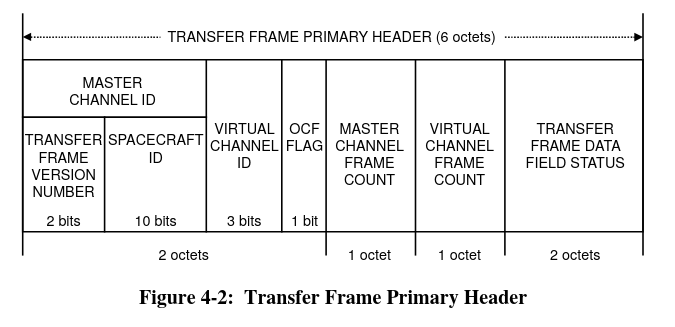
\includegraphics[width=10.5cm]{tmheader}
  \end{center}

  \emph{Hint:} Both the TM Space Data Link frames and AOS Space Data Link frames
  start by a Transfer Frame Version Number field. Its value can be used to
  distinguish them
\end{frame}

\handson{Brief look at the frames with Python: CRC's and headers}

\begin{frame}{About BepiColombo}
  BepiColombo's telemetry is very similar to Solar Orbiter

  \begin{center}
  \begin{tabular}{r | c | c}
    & {\bf Solar Orbiter} & {\bf BepiColombo} \\
    \hline
    {\bf Modulation} & PCM/PM/Bi-$\varphi$ & PCM/PM/Bi-$\varphi$ \\
    {\bf Baudrate} & 555.5k & 700k\\
    {\bf Coding} & $r = 1/2$ Turbo & $r = 1/2$ Turbo\\
    {\bf Frame size} & 8920 bits & 8920 bits\\
    {\bf Fames} & TM & TM \\
  \end{tabular}
  \end{center}

  The signal in the recording is weaker than Solar Orbiter's, so trying to
  decode is a good exercise to check decoder performance

  \medskip

  Most of the frames contain idle data, but they are interesting to analyze,
  because they are filled with a PN sequence that resets ``unexpectedly''
\end{frame}

\begin{frame}{Further reading}
  Mars spacecraft (in collaboration with AMSAT-DL and Bochum observatory)
  
  Just search in \url{http://destevez.net}
  
  \begin{center}
  \begin{tabular}{r | c | c | c }
    & {\bf EMM } & {\bf Tianwen-1} & {\bf Tianwen-1 (high-speed)} \\
    \hline
    {\bf Modulation} & PCM/PM/NRZ & PCM/PSK/PM & QPSK \\
    {\bf Baudrate} & 12k & 16384 &  2048k\\
    {\bf Coding} & $r = 1/6$ Turbo & Concatenated &  Concatenated \\
    {\bf Frame size} & 1784 bits & 1760 bits &  7136 bits \\
    {\bf Fames} & AOS & AOS &  AOS\\
  \end{tabular}
  \end{center}
  \begin{center}
  \begin{tabular}{r | c | c}
    & {\bf Mars 2020 (safe mode)} & {\bf Mars 2020} \\
    \hline
    {\bf Modulation} & PCM/PSK/PM & PCM/PM/NRZ \\
    {\bf Baudrate} & 80 & 60k \\
    {\bf Coding} & $r = 1/2$ Turbo & $r = 1/6$ Turbo \\
    {\bf Frame size} & 1784 bits & 8920 bits \\
    {\bf Fames} & AOS & AOS \\
  \end{tabular}
  \end{center}
\end{frame}

\begin{frame}
  \begin{block}{}
    \begin{center}
      \vspace{1em}
      {\huge Additional material}
      \vspace{1em}
    \end{center}
  \end{block}
\end{frame}

\begin{frame}{Two other approaches for Manchester demodulation}
  We have downconverted a sideband to baseband, which can also be used for
  PCM/PSK/PM. To demodulate Manchester, we can instead:
  \begin{itemize}
    \item Demodulate as twice the symbol rate, then use \emph{Manchester Sync}
      from gr-satellites to find and wipe the Manchester clock
    \item Use an FIR filter as matched filter to the Manchester pulse
  \end{itemize}

  \begin{center}
    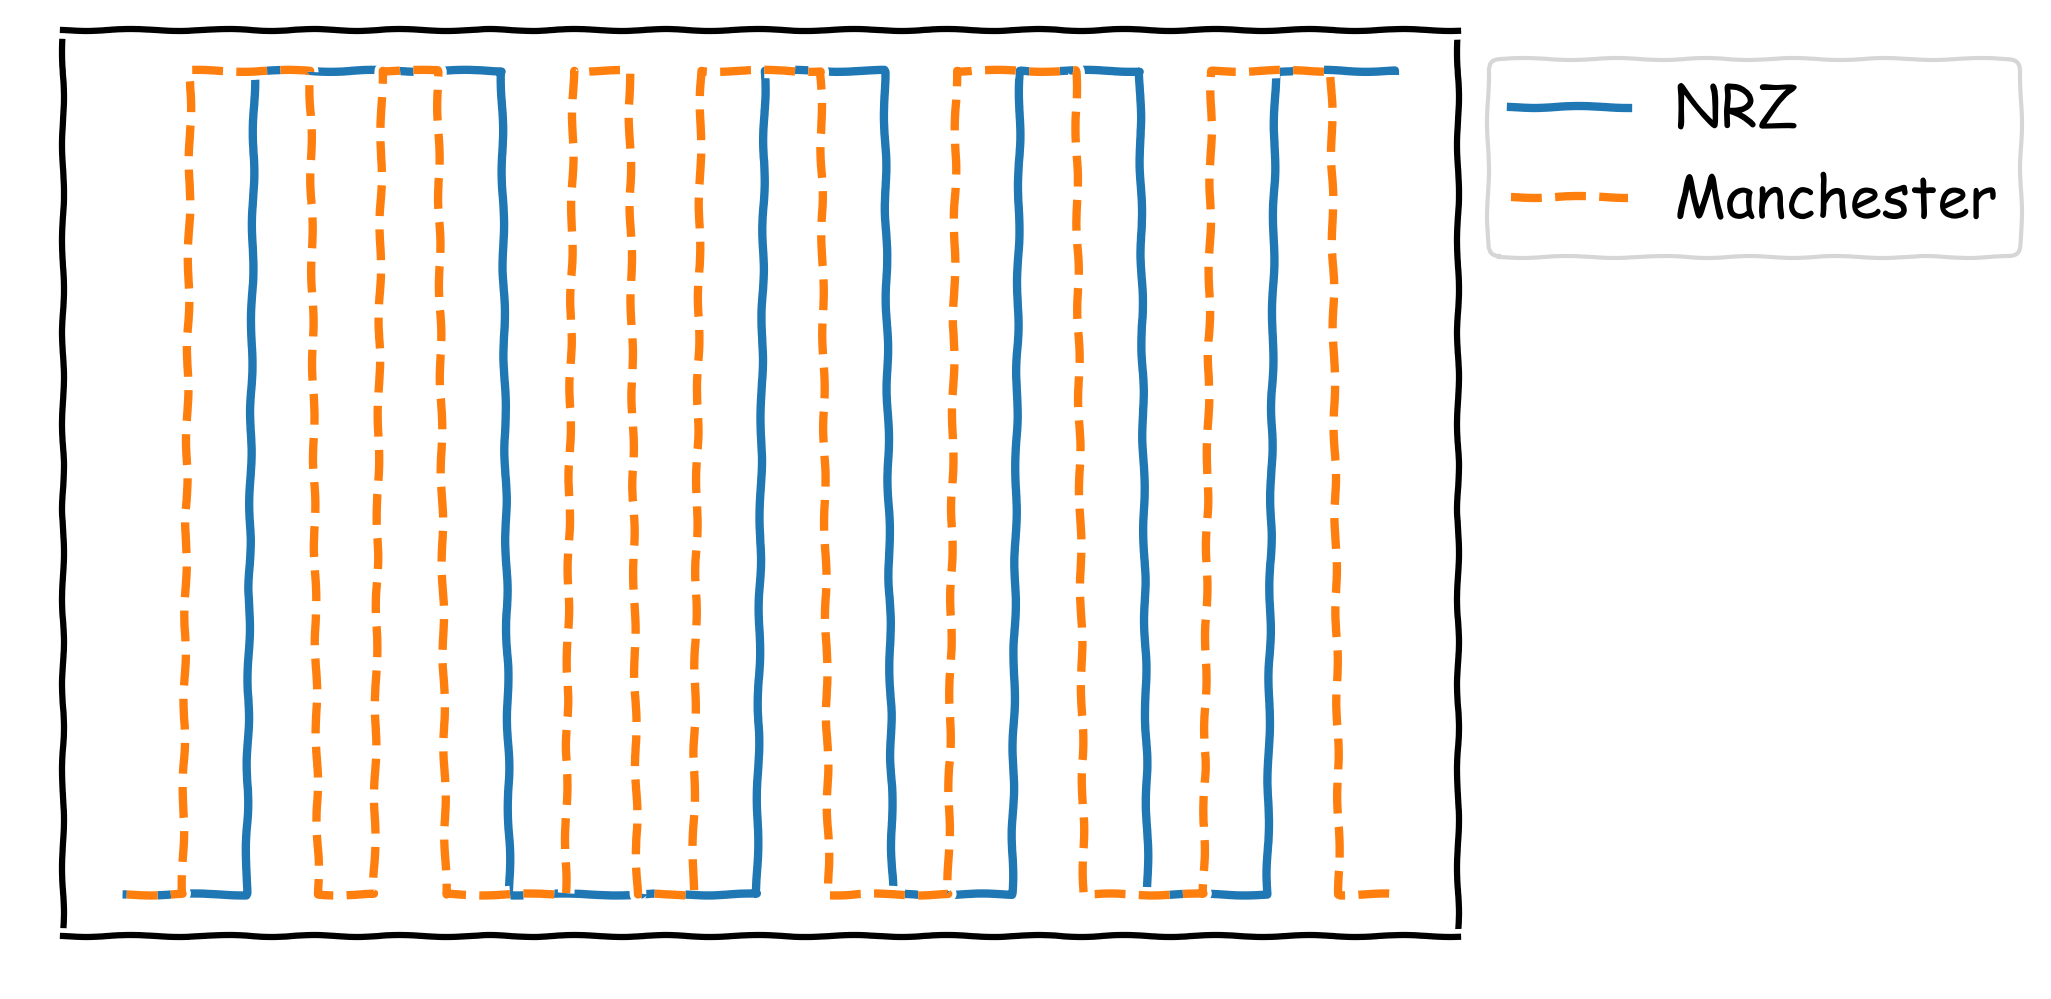
\includegraphics[width=9.5cm]{manchester_wave}
  \end{center}
\end{frame}

\begin{frame}{Manchester Sync}
  The \emph{Manchester sync} block gets an input at twice the symbol rate...
  \begin{center}
    \texttt{$\cdots$1 0 1 1 0 1 0 0 1 0 1 1 0 1 0 0 1 1 0 0 1 1 0 1 0$\cdots$}
  \end{center}
  ...finds the phase of the Manchester clock, by making pairs that look like
  \texttt{01} and \texttt{10}...
  \begin{center}
    \texttt{$\cdots$1|0 1|1 0|1 0|0 1|0 1|1 0|1 0|0 1|1 0|0 1|1 0|1 0$\cdots$}
  \end{center}
  ...and ``wipes'' the Manchester block, by replacing each Manchester pair by
  the corresponding NRZ symbol...
  \begin{center}
    \texttt{$\cdots$ | 0 | 1 | 1 | 0 | 0 | 1 | 1 | 0 | 1 | 0 | 1 | 1 $\cdots$}
  \end{center}
\end{frame}

\begin{frame}{Manchester pulse matched filter}
  If we use the Manchester pulse \texttt{10} as a matched filter, we wipe the
  Manchester clock and obtain the correct symbols at the optimal sampling
  locations.

  We also obtain spurious sampling locations between adjacent and equal symbols.
  \begin{center}
      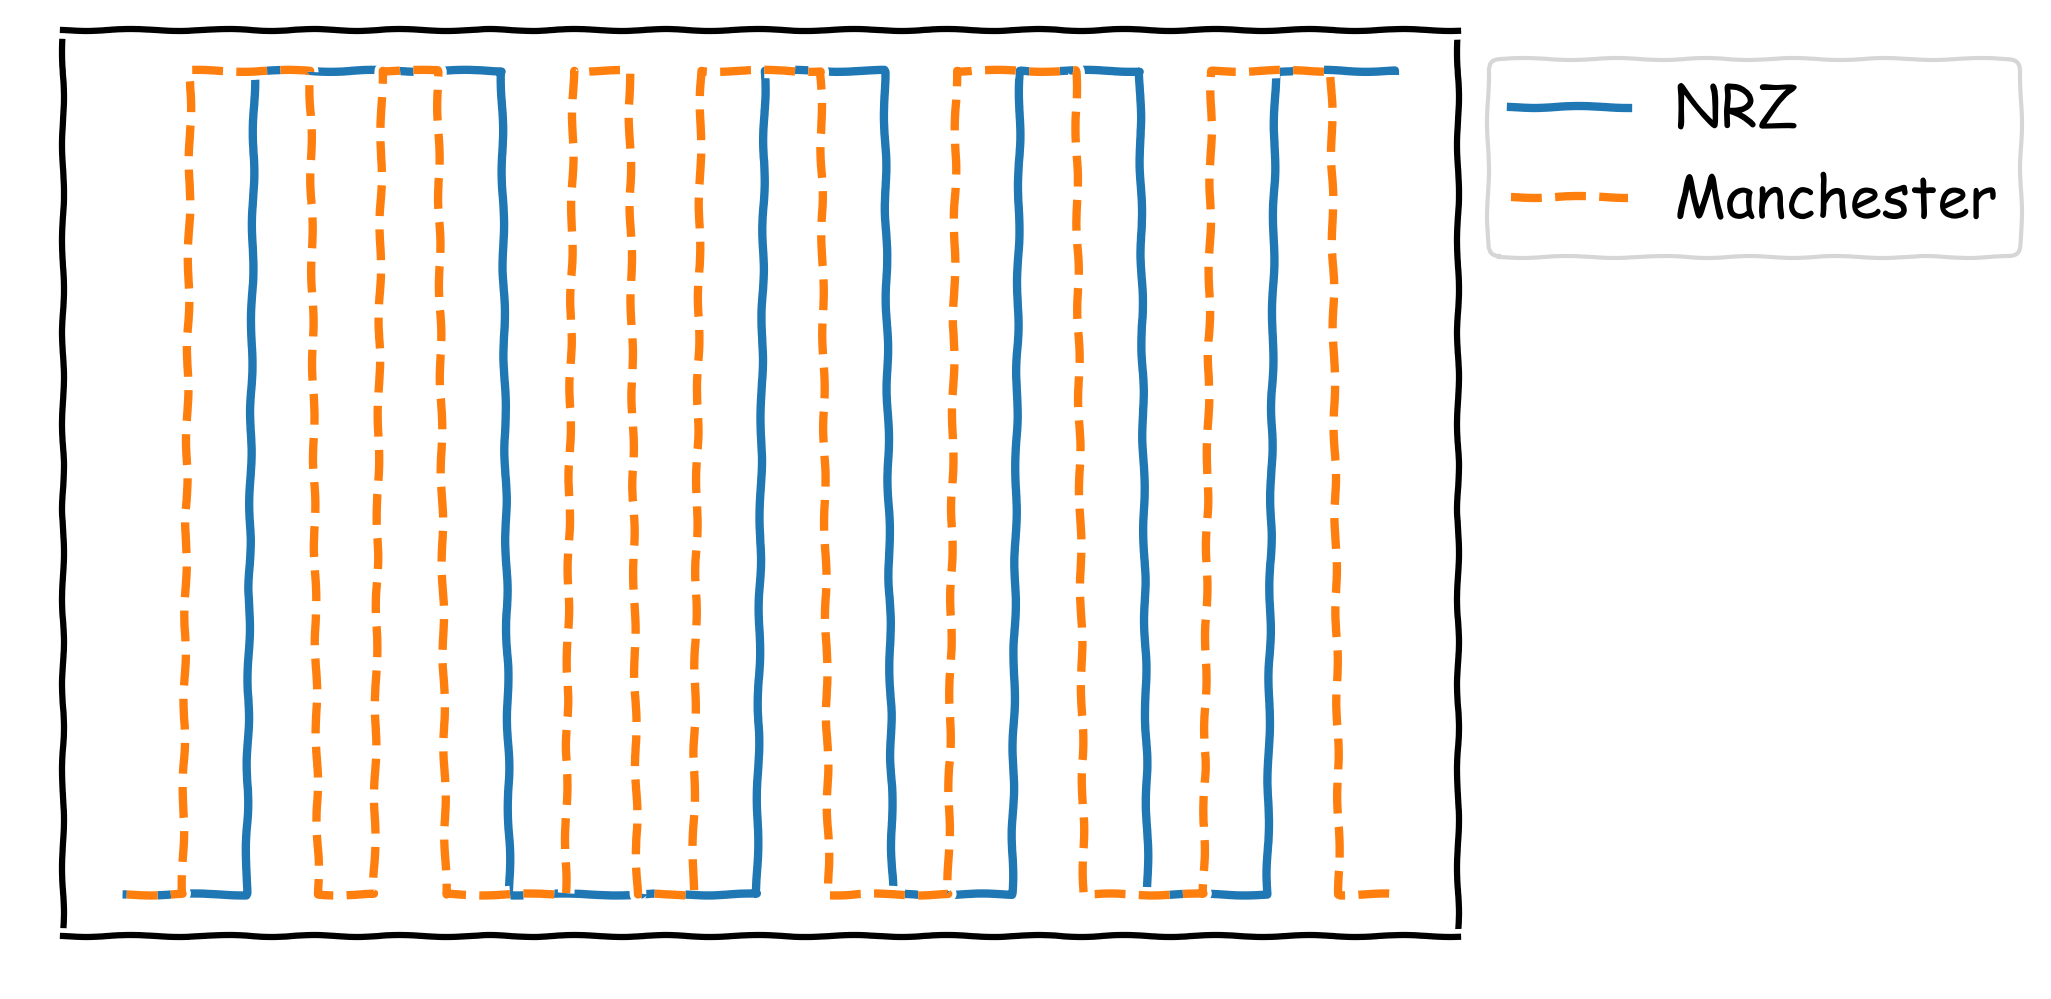
\includegraphics[width=7cm]{manchester_wave}
      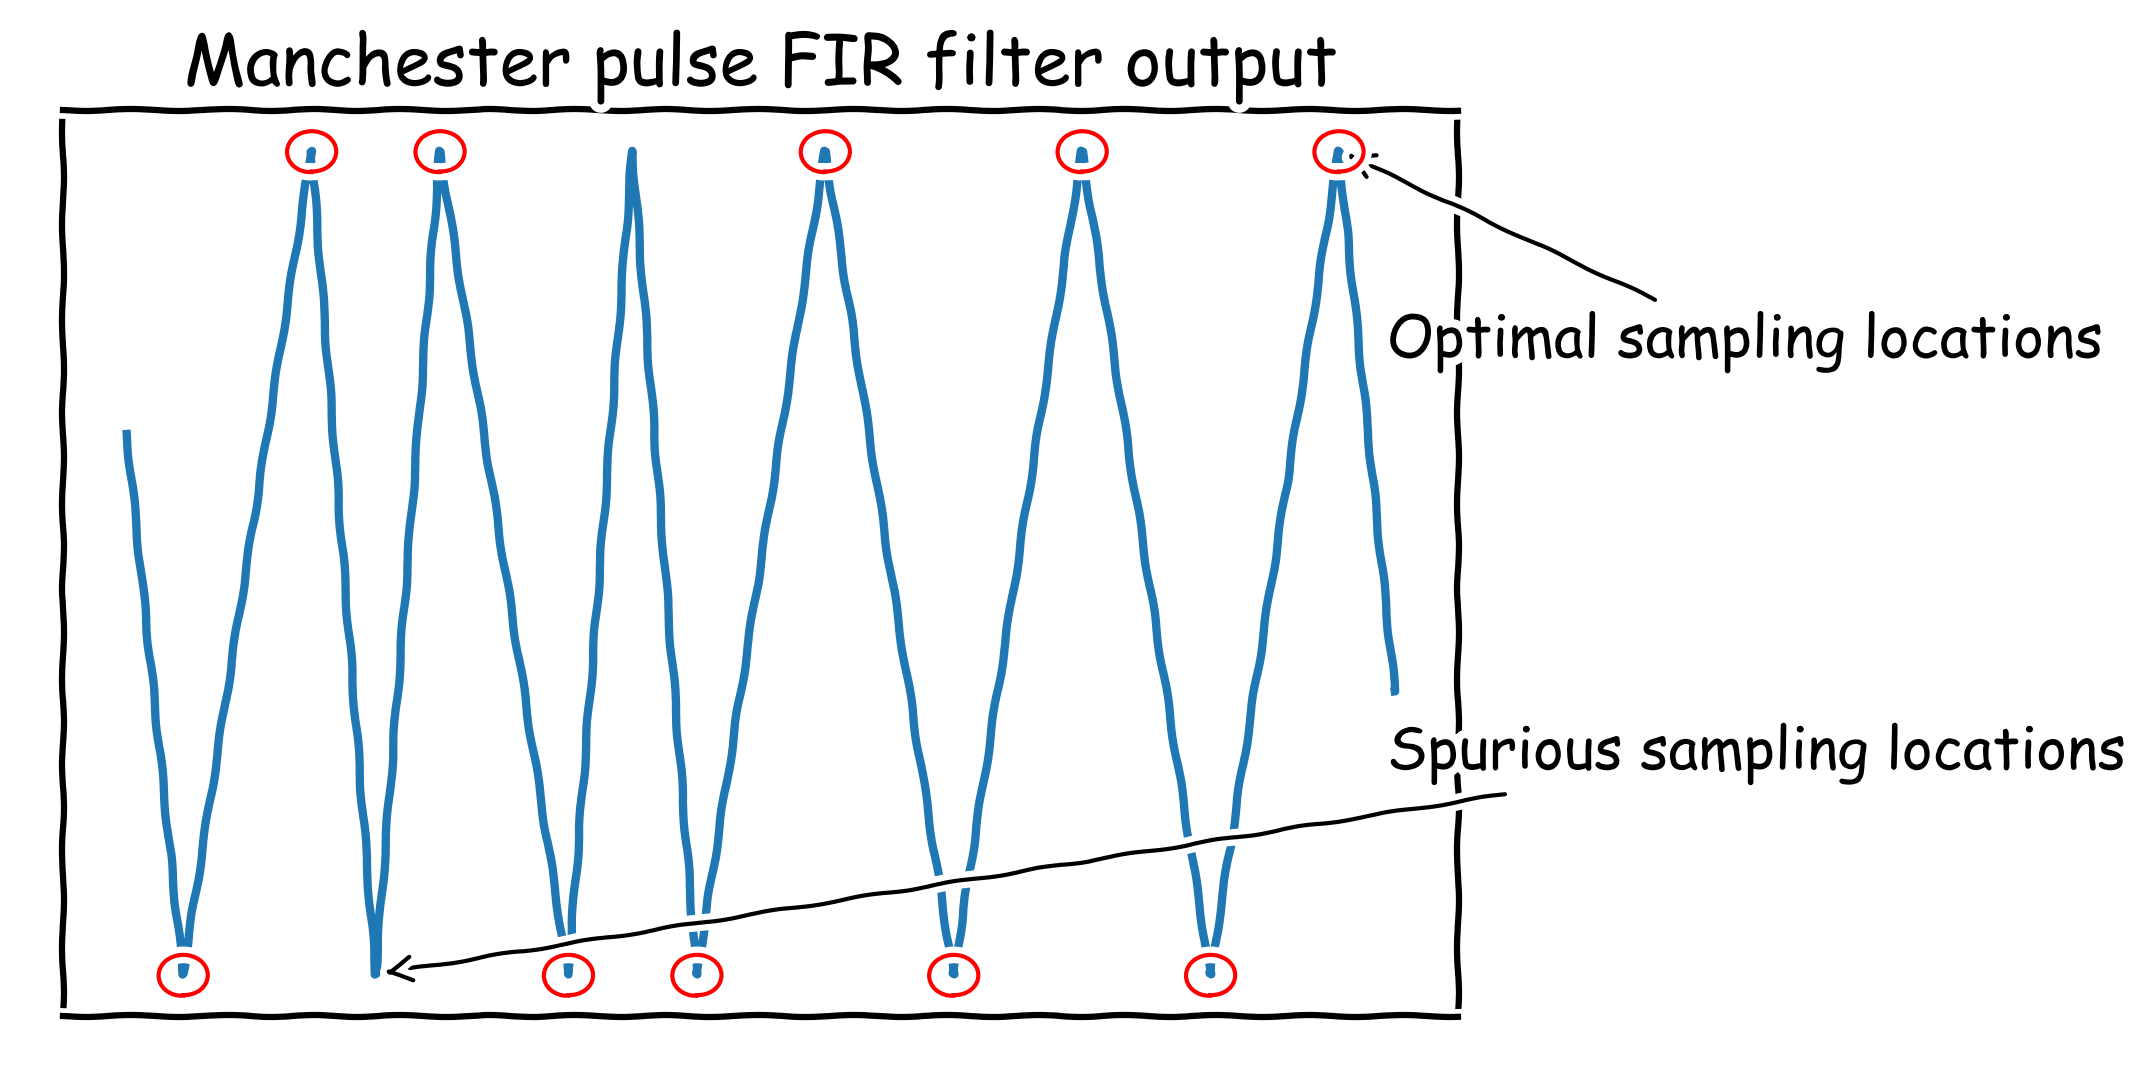
\includegraphics[width=7cm]{manchester_fir}
  \end{center}

  However, the clock phase for spurious sampling locations is unstable, so a
  DTLL (\emph{Symbol Sync}) will tend to lock to the correct optimal sampling
  locations phase.

  It is good to resample to an even samples-per-symbol before the FIR filter.
\end{frame}

% Structuring a talk is a difficult task and the following structure
% may not be suitable. Here are some rules that apply for this
% solution: 

% - Exactly two or three sections (other than the summary).
% - At *most* three subsections per section.
% - Talk about 30s to 2min per frame. So there should be between about
%   15 and 30 frames, all told.

% - A conference audience is likely to know very little of what you
%   are going to talk about. So *simplify*!
% - In a 20min talk, getting the main ideas across is hard
%   enough. Leave out details, even if it means being less precise than
%   you think necessary.
% - If you omit details that are vital to the proof/implementation,
%   just say so once. Everybody will be happy with that.


% \section{Motivation}
% 
% \subsection{The Basic Problem That We Studied}
% 
% \begin{frame}{Make Titles Informative. Use Uppercase Letters.}{Subtitles are optional.}
%   % - A title should summarize the slide in an understandable fashion
%   %   for anyone how does not follow everything on the slide itself.
% 
%   \begin{itemize}
%   \item
%     Use \texttt{itemize} a lot.
%   \item
%     Use very short sentences or short phrases.
%   \end{itemize}
% \end{frame}
% 
% \begin{frame}{Make Titles Informative.}
% 
%   You can create overlays\dots
%   \begin{itemize}
%   \item using the \texttt{pause} command:
%     \begin{itemize}
%     \item
%       First item.
%       \pause
%     \item    
%       Second item.
%     \end{itemize}
%   \item
%     using overlay specifications:
%     \begin{itemize}
%     \item<3->
%       First item.
%     \item<4->
%       Second item.
%     \end{itemize}
%   \item
%     using the general \texttt{uncover} command:
%     \begin{itemize}
%       \uncover<5->{\item
%         First item.}
%       \uncover<6->{\item
%         Second item.}
%     \end{itemize}
%   \end{itemize}
% \end{frame}
% 
% 
% \subsection{Previous Work}
% 
% \begin{frame}{Make Titles Informative.}
% \end{frame}
% 
% \begin{frame}{Make Titles Informative.}
% \end{frame}
% 
% 
% 
% \section{Our Results/Contribution}
% 
% \subsection{Main Results}
% 
% \begin{frame}{Make Titles Informative.}
% \end{frame}
% 
% \begin{frame}{Make Titles Informative.}
% \end{frame}
% 
% \begin{frame}{Make Titles Informative.}
% \end{frame}
% 
% 
% \subsection{Basic Ideas for Proofs/Implementation}
% 
% \begin{frame}{Make Titles Informative.}
% \end{frame}
% 
% \begin{frame}{Make Titles Informative.}
% \end{frame}
% 
% \begin{frame}{Make Titles Informative.}
% \end{frame}
% 
% 
% 
% \section*{Summary}
% 
% \begin{frame}{Summary}
% 
%   % Keep the summary *very short*.
%   \begin{itemize}
%   \item
%     The \alert{first main message} of your talk in one or two lines.
%   \item
%     The \alert{second main message} of your talk in one or two lines.
%   \item
%     Perhaps a \alert{third message}, but not more than that.
%   \end{itemize}
%   
%   % The following outlook is optional.
%   \vskip0pt plus.5fill
%   \begin{itemize}
%   \item
%     Outlook
%     \begin{itemize}
%     \item
%       Something you haven't solved.
%     \item
%       Something else you haven't solved.
%     \end{itemize}
%   \end{itemize}
% \end{frame}
% 
% 
% 
% % All of the following is optional and typically not needed. 
% \appendix
% \section<presentation>*{\appendixname}
% \subsection<presentation>*{For Further Reading}
% 
% \begin{frame}[allowframebreaks]
%   \frametitle<presentation>{For Further Reading}
%     
%   \begin{thebibliography}{10}
%     
%   \beamertemplatebookbibitems
%   % Start with overview books.
% 
%   \bibitem{Author1990}
%     A.~Author.
%     \newblock {\em Handbook of Everything}.
%     \newblock Some Press, 1990.
%  
%     
%   \beamertemplatearticlebibitems
%   % Followed by interesting articles. Keep the list short. 
% 
%   \bibitem{Someone2000}
%     S.~Someone.
%     \newblock On this and that.
%     \newblock {\em Journal of This and That}, 2(1):50--100,
%     2000.
%   \end{thebibliography}
% \end{frame}

\end{document}


